% \documentclass[a4paper,10pt]{article}
\documentclass[review]{siamart}
\usepackage{url}
\usepackage{amssymb}
\usepackage{amsmath}
\usepackage{bm}
\usepackage{stmaryrd}
\usepackage{array}
\usepackage{multirow}
\usepackage{empheq}
\usepackage{enumitem}
	\setlist{nosep} % or \setlist{noitemsep} to leave space around whole list
\usepackage{color}
\usepackage{verbatim}
% \usepackage{showlabels}
\usepackage{stmaryrd}
\usepackage{adjustbox}
\usepackage{hyperref}
\definecolor{darkgreen}{rgb}{0.0, 0.5, 0}
\usepackage[numbers,sort]{natbib}
\usepackage{cleveref}
\usepackage[belowskip=-5pt]{subcaption}
\usepackage{grffile}

\newsiamremark{remark}{Remark}
\newsiamremark{assumption}{Assumption}


% \newtheorem{lemma}{Lemma}
% \newtheorem{definition}{Definition}
% \newtheorem{theorem}{Theorem}
% \newtheorem{corollary}{Corollary}

\newcommand{\tcb}{\textcolor{blue}}
\newcommand{\tcp}{\textcolor{purple}}
\newcommand{\todo}[1]{\textcolor{red}{[TODO\@: #1]}}

\newcommand{\mdet}{\operatorname{det}}
\newcommand{\madj}{\operatorname{adj}}

% ------------------------------------------------------------------------------------ %
% ------------------------------------------------------------------------------------ %

\newcommand{\TheTitle}{Fast parallel solution of fully implicit Runge-Kutta and discontinuous
	Galerkin in time for numerical PDEs, Part I: the linear setting}
\newcommand{\TheAuthors}{B.S. Southworth, O.A. Krzysik, W. Pazner, and H. De Sterck}
\headers{Parallel solution of fully implict Runge-Kutta and DG in time I}{\TheAuthors}
\title{{\TheTitle}\thanks{This research was conducted ...
  }}

\author{
	Ben S. Southworth\thanks{Department of Applied Mathematics,
    University of Colorado,
    U.S.A. (\url{ben.s.southworth@gmail.com}),
    \url{http://orcid.org/0000-0002-0283-4928}}
\and
    Oliver A. Krzysik\thanks{School of Mathematics, Monash University,
  	Australia (\url{oliver.krzysik@monash.edu}),
  	\url{https://orcid.org/0000-0001-7880-6512}}
\and
  	Will Pazner\thanks{Center for Applied Scientific Computing, Lawrence Livermore National Laboratory,
    U.S.A. (\url{pazner1@llnl.gov})}
\and
    Hans De Sterck\thanks{Department of Applied Mathematics,
  	University of Waterloo,
  	Waterloo, Canada
  	(\url{hdesterck@uwaterloo.ca})}
}

\ifpdf%
\hypersetup{%
  pdftitle={\TheTitle},
  pdfauthor={\TheAuthors}
}
\fi

% ------------------------------------------------------------------------------------ %
% ------------------------------------------------------------------------------------ %

\begin{document}
\maketitle
\allowdisplaybreaks

\begin{abstract}

\end{abstract}


% ------------------------------------------------------------------------------------- %
% ------------------------------------------------------------------------------------- %
% ------------------------------------------------------------------------------------- %
\section{Introduction}\label{sec:intro}

% ------------------------------------------------------------------------------------- %
% ------------------------------------------------------------------------------------- %
\subsection{Fully implicit Runge-Kutta}\label{sec:intro:irk}

Consider the method-of-lines approach to the numerical solution of linear
partial differential equations (PDEs), where we discretize in space and arrive
at a system of ordinary differential equations (ODEs) in time,
%
\begin{align}\label{eq:problem}
M\mathbf{u}'(t) =  \mathcal{L}(t)\mathbf{u} + \mathbf{f}(t)
	\quad\text{in }(0,T], \quad \mathbf{u}(0) = \mathbf{u}_0,
\end{align}
%
where $M$ is a mass matrix, $\mathcal{L}(t)\in\mathbb{R}^{N\times N}$ a discrete
linear operator, and $\mathbf{f}(t)$ a time-dependent forcing
function.\footnote{Note,
PDEs with an algebraic constraint, for example, the divergence-free
constraint in incompressible Navier Stokes, instead yield a differential algebraic equation (DAE), which
requires separate careful treatment and will be the subject of a forthcoming paper.}
Then, consider time propagation using an $s$-stage Runge-Kutta scheme,
characterized by the Butcher tableau
%
\begin{align*}
	\renewcommand\arraystretch{1.2}
	\begin{array}
	{c|c}
	\mathbf{c}_0 & A_0\\
	\hline
	& \mathbf{b}_0^T
	\end{array},
\end{align*}
%
with Runge-Kutta matrix $A_0 = (a_{ij})$, weight vector $\mathbf{b}_0^T = (b_1,
\ldots, b_s)^T$, and quadrature nodes $\mathbf{c}_0 = (c_0, \ldots, c_s)$.

Runge-Kutta methods update the solution using a sum over stage vectors,
%
\begin{align}\label{eq:update}
\mathbf{u}_{n+1} & = \mathbf{u}_n + \delta t \sum_{i=1}^s b_i\mathbf{k}_i, \\
M\mathbf{k}_i & = \mathcal{L}(t_n+\delta tc_i)\cdot
	\left(\mathbf{u}_n + \delta t\sum_{j=1}^s a_{ij}\mathbf{k}_j\right) +
	\mathbf{f}(t_n+\delta tc_i).\label{eq:stages}
\end{align}
%
Expanding, solving for the stage vectors $\{\mathbf{k}_i\}$ can then be expressed
as the solution of the block linear system,
%
\begin{align}\label{eq:k0}
\left( \begin{bmatrix} M  & & \mathbf{0} \\ & \ddots \\ \mathbf{0} & & M\end{bmatrix}
	- \delta t \begin{bmatrix} a_{11}\mathcal{L}_1 & ... & a_{1s}\mathcal{L}_1 \\
	\vdots & \ddots & \vdots \\ a_{s1}\mathcal{L}_s & ... & a_{ss} \mathcal{L}_s \end{bmatrix} \right)
	\begin{bmatrix} \mathbf{k}_1 \\ \vdots \\ \mathbf{k}_s \end{bmatrix}
& = \begin{bmatrix} \mathbf{f}_1 \\ \vdots \\ \mathbf{f}_s \end{bmatrix},
\end{align}
%
where $\mathcal{L}_i := \mathcal{L}(t_n+\delta tc_i)$ and $\mathbf{f}_i :=
\mathbf{f}(t_n+\delta tc_i)$. Primarily this paper
focuses on spatial operators that are independent of time; however, some of
the results hold for commuting operators, such as may arise in, for example,
a time-dependent reaction term, so for now we maintain this generality.

The difficulty in fully implicit Runge-Kutta methods (which we will denote IRK) lies in
solving the $Ns\times Ns$ block linear system in \eqref{eq:k0}. This paper focuses on the
parallel simulation of numerical PDEs, where $N$ is typically very large
and $\mathcal{L}$ is highly ill-conditioned. In such cases, direct
solution techniques to solve \eqref{eq:k0} are not a viable option, and fast, parallel
iterative methods must be used. However, IRK methods are rarely employed in practice due
to the difficulties of solving \eqref{eq:k0}. Even for relatively simple
parabolic PDEs where $\mathcal{L}$ is symmetric positive definite (SPD), \eqref{eq:k0}
instead yields a large nonsymmetric system with significant block coupling. For
nonsymmetric systems $\mathcal{L}$ that already have variable coupling, fast iterative
methods are even less likely to yield acceptable performance in solving \eqref{eq:k0}.

% ------------------------------------------------------------------------------------- %
% ------------------------------------------------------------------------------------- %
\subsection{Discontinuous Galerkin in time}\label{sec:intro:dg}

The use of finite element and Galerkin methods for the temporal discretization of numerical PDEs has seen growing interest.
Some of the more interesting features of using finite elements in time is the natural ability to handle time-dependent geometries, unstructured space-time meshes, and both spatial and temporal adaptive mesh refinement.
However, for so-called slab-based meshing in time with discontinuous Galerkin (DG) finite elements, where the time domain is discretized using spatial slabs (that is, the same time step is applied to the entire spatial domain, analogous to more traditional method of lines time-stepping techniques), the resulting linear systems that must be solved for each time step take the same structure as \eqref{eq:k0} (for example, see \cite{hn,Akrivis2011}).
In fact, for specific choices of quadrature, discontinuous Galerkin time discretizations are equivalent to certain collocation Runge-Kutta methods \cite{Lasaint1974}.
A handful of works have looked at linear solvers for such discretizations, primarily for parabolic problems, including block preconditioning approaches \cite{exh,8jp,27n}, and direct space-time multigrid methods \cite{gander2016analysis}.

Although this paper focuses on fully implicit Runge-Kutta, the algorithms developed here can also be applied to DG discretizations in time on fixed slab-based meshes.
In fact, some of the principles used in this paper are similar to those used in \cite{exh} for space-time DG discretizations of linear parabolic problems, and some of the theory derived therein is generalized to non-parabolic/non-SPD operators in this paper.

% ------------------------------------------------------------------------------------- %
% ------------------------------------------------------------------------------------- %
\subsection{Outline}\label{sec:intro:outline}

This paper develops fast, parallel preconditioning techniques for the solution of
fully implicit Runge-Kutta methods and DG discretizations in time
for linear numerical PDEs.
First, \Cref{sec:intro:hist} provides background on why IRK methods are desirable
over the simpler and more commonly used DIRK methods, and also provides some
historical context for the preconditioners developed in this work.
\Cref{sec:intro:stab} then briefly discusses stable integration from
a method-of-lines perspective and introduces two key elements that will be
used throughout the paper.

\Cref{sec:solve} introduces a new method to solve for the IRK update
\eqref{eq:update} for linear operators $\mathcal{L}$ that are independent of time.
The new method effectively
requires the preconditioning of $s$ real-valued matrices along the lines of
$\eta M - \delta t\mathcal{L}$, for some $\eta > 1$, and is easily implemented
using existing preconditioners and parallel software libraries.
In contrast to other works that have considered the preconditioning of \eqref{eq:kron1},
the proposed algorithm here (i) is amenable to short-term Krylov recursion (conjugate
gradient (CG)/MINRES) if $\eta M - \mathcal{L}$ is, and (ii) only operates on the solution,
thus not requiring the storage of each stage vector. Theory is developed
that guarantees rapid convergence of GMRES and CG under basic assumptions
on stability from \Cref{sec:intro:stab} (see \Cref{sec:solve:prec}). A slight
modification of the method is then developed, and the resulting preconditioned
operator is proven to have condition number $<9$ (and typically $\sim1-4$ for
realistic parameters), independent of the number of
stages/polynomial order in time (see \Cref{sec:solve:gamma}).

Numerical results are provided in \Cref{sec:numerics}, demonstrating the new
method for a variety of problems and corresponding preconditioners, including
high-order finite-difference and DG (spatial) discretizations of
advection(-diffusion), and very high-order matrix-free continuous Galerkin
discretizations of diffusion. The method is shown to be fast and scalable
up to 10th-order accuracy in time, effective on fully advective (hyperbolic)
problems, and, for one example, can obtain 4th-order accuracy with Gauss
integration using roughly half the algebraic multigrid (AMG) iterations
as needed by standard 4th-order SDIRK schemes.

% ------------------------------------------------------------------------------------- %
% ------------------------------------------------------------------------------------- %
\subsection{Why fully implicit and previous work}\label{sec:intro:hist}

In practice, people typically use
diagonally implicit Runge-Kutta (DIRK) methods, where $A_0$ is lower triangular.
For such schemes, the solution of \eqref{eq:k0} only requires $s$ linear
solves along the lines of $ M - \delta ta_{ii}\mathcal{L}_i$. Unfortunately, DIRK
schemes suffer from stage-order one (stage-order two with one explicit stage; see
EDIRK methods \cite{butcher00}). For stiff nonlinear PDEs or DAEs, the observed
global order of accuracy
in practice can be limited to $\approx \min\{ p, q+1\}$ or $q$, respectively, for
integration order $p$ and stage-order $q$ \cite{hairer96,kennedy16}. Thus, even a
6th-order DIRK method may only yield 1st- or 2nd-order accuracy. In contrast, IRK
methods yield high stage order and, thus, formally high-order accuracy on stiff,
nonlinear problems, and even index-2 DAEs. Although the focus of this paper is
linear PDEs with no algebraic constraint, we want to highlight that the theory
and framework developed here is fundamental to a forthcoming paper on
nonlinear PDEs and DAEs. Furthermore, for less stiff
problems, IRK methods can yield accuracy as high as order $2s$ for an $s$ stage method,
compared with a maximum of $s$ or $s+1$ for SDIRK methods with reasonable stability
properties \cite[Section IV.6]{hairer96}.

One simplification for using IRK methods is to assume $\mathcal{L}_i =
\mathcal{L}_j$ for all $i,j$, in which case \eqref{eq:k0} can be expressed in
Kronecker product form,
%
\begin{align}\label{eq:kron1}
(I\otimes M - \delta t A_0\otimes \mathcal{L})\mathbf{k} & = \mathbf{f}.
\end{align}
%
Such an assumption is natural for linear problems with no time-dependent differential
components and, for the most part, covers the type of problems studied in this paper.
Many papers have considered the solution of \eqref{eq:kron1}, with Butcher
\cite{butcher76} and Bickart's \cite{bickart77} being some of the earliest works,
which develop ways to transform \eqref{eq:kron1} to a simpler form.\footnote{
In Kronecker form \eqref{eq:kron1}, SIRK methods \cite{norsett1976runge} are also
relatively straightforward to solve using existing preconditioning techniques.
But, although SIRK method offer some advantages over DIRK methods, they still lack
the favorable stability and accuracy properties of IRK methods \cite{burrage82,orel91}.}
There, and in many of the works that followed, the goal was to minimize the cost of LU
decompositions used to solve \eqref{eq:kron1}, typically in the context of ODEs.

For large-scale simulation of PDEs, particularly on modern computing architectures,
LU decompositions (or other direct inverses) are typically not feasible. In this
vein, a number of people have considered preconditioning techniques for \eqref{eq:kron1}
or approximations to \eqref{eq:kron1} on the nonlinear iteration level or time
discretization level. In addition to the DG-in-time methods discussed in
\Cref{sec:intro:dg}, various block preconditioning/approximation techniques
have been studied, primarily for parabolic problems
\cite{houwen97b,Houwen97c,nissen11,mardel07,staff06,hoffmann97,jay00}, and
multigrid methods for IRK and parabolic problems were developed in \cite{vanlent05}.
New ADI-type preconditioners for IRK methods were developed for parabolic problems
in \cite{chen14} with spectral radius shown to be $<1$ under reasonable assumptions,
and the method extended to the viscous wave equation in first-order form in
\cite{chen16}. More recently, block-ILU preconditioners were successfully applied
to a transformed version of \eqref{eq:kron1} in \cite{pazner17} on more difficult
nonlinear compressible fluids problems.

Despite many papers considering the efficient solution of IRK methods, very little
has been done in the development and analysis of preconditioning techniques for
non-parabolic problems/non-SPD spatial operators, particularly methods that are
amenable to combine with existing fast, parallel preconditioners. Addressing each
of these challenges for linear PDEs is the focus of this work.

% ------------------------------------------------------------------------------------- %
% ------------------------------------------------------------------------------------- %
\subsection{A preconditioning framework and stability}\label{sec:intro:stab}

Throughout the paper, we use the reformulation used in, for example,
\cite{pazner17}, where we can pull an $A_0\otimes I$ out of the
fully implicit system in \eqref{eq:k0}, yielding the equivalent problem
%
\begin{align}\label{eq:keq}
\left( A_0^{-1}\otimes M - \delta t \begin{bmatrix} \mathcal{L}_1  & \\ & \ddots \\ && \mathcal{L}_s\end{bmatrix}\right)
	(A_0\otimes I)	\begin{bmatrix} \mathbf{k}_1 \\ \vdots \\ \mathbf{k}_s \end{bmatrix}
& = \begin{bmatrix} \mathbf{f}_1 \\ \vdots \\ \mathbf{f}_s \end{bmatrix}.
\end{align}
%
The off-diagonal block coupling in \eqref{eq:keq} now consists of mass matrices
rather than differential operators, which makes the analysis and solution more
tractable.
The algorithms developed here depend on the eigenvalues of $A_0$ and
$A_0^{-1}$, leading to our first assumption.
%
\begin{assumption}\label{ass:eig}
Assume that all eigenvalues of $A_0$ have positive real part.
\end{assumption}
%
Recall that if an IRK method is A-stable, irreducible, and $A_0$ is invertible
(which includes Gauss, Radau IIA, and Lobatto IIIC integration, among others),
then \Cref{ass:eig} holds \cite{hairer96}; that is, this assumption is
straightforward to satisfy in practice.

Stability must be taken into consideration when applying ODE solvers within a
method-of-lines approach to numerical PDEs. The Dalhquist test problem extends
naturally to this setting, where we are interested in the stability of the
linearized operator $\mathcal{L}$, for the ODE(s)
$\mathbf{u}'(t) = \mathcal{L}\mathbf{u}$, with solution $e^{t\mathcal{L}}\mathbf{u}$.
A necessary condition for stability is that the eigenvalues of $\mathcal{L}$
lie within distance $\mathcal{O}(\delta t)$ of the region of stability for
the Runge-Kutta scheme of choice (e.g., see \cite{reddy92}). Here we are
interested in implicit schemes and, because the majority of implicit Runge-Kutta schemes
used in practice are A- or L-stable, an effectively necessary condition for
stability is that the eigenvalues of $\mathcal{L}$ be nonpositive. For
normal operators, this requirement ends up being a necessary and sufficient
condition for stability.

For non-normal or non-diagonalizable operators, the analysis is more complicated.
One of the best known works on the subject is by Reddy and Trefethen \cite{reddy92},
where necessary and sufficient conditions for stability are derived as the
$\varepsilon$ pseudo-eigenvalues of $\mathcal{L}$ being within
$\mathcal{O}(\varepsilon) + \mathcal{O}(\delta t)$ of the stability region
as $\varepsilon,\delta t\to 0$. Here we relax this assumption to something
that is more tractable to work with by noting that the $\varepsilon$
pseudo-eigenvalues are contained within the field of values to
$\mathcal{O}(\varepsilon)$ \cite[Eq. (17.9)]{trefethen2005spectra},
where the field of values is defined as
%
\begin{align}\label{eq:fov}
W(\mathcal{L}) := \left\{ \langle \mathcal{L}\mathbf{x},\mathbf{x}\rangle \text{ : }
	\|\mathbf{x}\| = 1 \right\}.
\end{align}
%
This motivates the following assumption for the analysis done in this paper.
%
\begin{assumption}\label{ass:fov}
Let $\mathcal{L}$ be the linear spatial operator, and assume that $W(\mathcal{L}) \leq 0$.
\end{assumption}
%
It should be noted that the field of values has an additional connection
to stability. From \cite[Theorem 17.1]{trefethen2005spectra}, we have that
$\|e^{t\mathcal{L}}\|\leq 1$ for all $t\geq 0$ if and only if $W(\mathcal{L}) \leq 0$.
This is analogous to the ``strong stability'' discussed by Leveque
\cite[Chapter 9.5]{leveque2007finite}, as opposed to the weaker (but still
sufficient) condition $\|e^{t\mathcal{L}}\|\leq C$ for all $t\geq 0$ and
some constant $C$. In practice, \Cref{ass:fov} is likely to hold when
simulating numerical PDEs, and in \Cref{sec:solve:prec}, it is proven that
\Cref{ass:eig} and \ref{ass:fov} provide sufficient conditions to guarantee
fast Krylov convergence of the proposed methods.

% ------------------------------------------------------------------------------------- %
% ------------------------------------------------------------------------------------- %
% ------------------------------------------------------------------------------------- %
\section{Fast parallel preconditioning}\label{sec:solve}

For ease of notation, let us scale both sides of \eqref{eq:keq} by a
block-diagonal mass matrix inverse, and let
%
\begin{equation*}
\widehat{\mathcal{L}}_i := \delta t M^{-1}\mathcal{L}_i,
\end{equation*}
%
for $i=1,..,s$. Now let $\alpha_{ij}$ denote the $ij$-element
of $A_0^{-1}$.\footnote{Note, there are
methods with one explicit stage followed by several fully implicit stages \cite{butcher00}.
In such cases, $A_0$ is not invertible, but the explicit stage can
be eliminated from the system (by doing an explicit time step). The remaining operator
can then be reformulated as in \eqref{eq:keq}.}
Then, solving \eqref{eq:k0} can be effectively reduced to inverting the operator
%
\begin{align}\nonumber
\mathcal{M}_s & := A_0^{-1}\otimes I - \begin{bmatrix} \widehat{\mathcal{L}}_1  & \\ & \ddots \\ && \widehat{\mathcal{L}}_s\end{bmatrix} \\
& = \begin{bmatrix} \alpha_{11}I - \widehat{\mathcal{L}}_1 & \alpha_{12}I & ... & \alpha_{1s}I \\
	\alpha_{21}I & \alpha_{22}I - \widehat{\mathcal{L}}_2 & & \alpha_{2s}I \\
	\ddots & & \ddots & \vdots \\ \alpha_{s1}I & ... & \alpha_{s(s-1)}I & \alpha_{ss}I - \widehat{\mathcal{L}}_s \end{bmatrix}.
	\label{eq:k1}
\end{align}
%
We proceed by deriving a closed form inverse of \eqref{eq:k1}, demonstrating
how the Runge-Kutta update in \eqref{eq:update} can then be performed directly
(without forming and saving each stage vector), and developing a preconditioning
strategy to apply this update using existing preconditioners.

% ------------------------------------------------------------------------------------- %
% ------------------------------------------------------------------------------------- %
\subsection{An inverse and update for commuting operators}\label{sec:solve:inv}

This section introduces a result similar to Bickart's \cite{bickart77},
but using a different framework and generalized to hold for commuting
operators. We consider $\mathcal{M}_s$ as a matrix over the commutative
ring of linear combinations of $\{I, \widehat{\widehat{\mathcal{L}}}\}$,
and the determinant and adjugate referred to in \Cref{lem:inv} are defined
over matrix-valued elements rather than scalars.

%
\begin{lemma}\label{lem:inv}
Let $\alpha_{ij}$ denote the $(i,j)$th entry of $A_0^{-1}$ and assume
$\{\widehat{\mathcal{L}}_i\}_{i=1}^s$ are commuting operators. Define $\mathcal{M}_s$
% \begin{align*}
% \mathcal{M}_s := \begin{bmatrix} \alpha_{11}I - \widehat{\mathcal{L}}_1 & \alpha_{12}I & ... & \alpha_{1s}I \\
% 	\alpha_{21}I & \alpha_{22}I - \widehat{\mathcal{L}}_2 & & \alpha_{2s}I \\
% 	\ddots & & \ddots & \vdots \\ \alpha_{s1}I & ... & \alpha_{s(s-1)}I & \alpha_{ss}I - \widehat{\mathcal{L}}_s \end{bmatrix},
% \end{align*}
as in \eqref{eq:k1},
let det$(\mathcal{M}_s)$ be the determinant of $\mathcal{M}_s$ (in this case a block-diagonal
matrix), and let adj$(\mathcal{M}_s)$ be the adjugate of $\mathcal{M}_s$. Then, $\mathcal{M}_s$
is invertible if and only if det$(\mathcal{M}_s)$ is invertible, and
\begin{align*}
\mathcal{M}_s^{-1} = \textnormal{det}(\mathcal{M}_s)^{-1}\textnormal{adj}(\mathcal{M}_s).
\end{align*}
%

Now, suppose $\widehat{\mathcal{L}}_i = \widehat{\mathcal{L}}_j$ for
all $i,j$, and let $P_s(x)$ be the characteristic polynomial of $A_0^{-1}$. Then,
\begin{align*}
\mathcal{M}_s^{-1} = \textnormal{diag}(P_s(\widehat{\mathcal{L}})^{-1})\textnormal{adj}(\mathcal{M}_s),
\end{align*}
where ``diag'' indicates a block diagonal matrix, with diagonal blocks given by $P_s(\widehat{\mathcal{L}})^{-1}$.
\end{lemma}
%
\begin{proof}
Notice in \eqref{eq:k1} that if $\widehat{\mathcal{L}}_i$ and $\widehat{\mathcal{L}}_j$ commute for all $i,j$,
then $\mathcal{M}_s$ is a matrix over the commutative ring of linear combinations
of $I$ and $\{\widehat{\mathcal{L}}_i\}$. Let adj$(\mathcal{M}_s)$ denote the matrix adjugate. A
classical result in matrix analysis tells us that
%
\begin{align*}
\textnormal{adj}(\mathcal{M}_s)\mathcal{M}_s = \mathcal{M}_s\textnormal{adj}(\mathcal{M}_s)
	= \textnormal{det}(\mathcal{M}_s)I.
\end{align*}
%
Moreover, $\mathcal{M}_s$ is invertible if and only if the determinant of $\mathcal{M}_s$
is invertible, in which case $\mathcal{M}_s^{-1} := $ det$(\mathcal{M}_s)^{-1}$adj$(\mathcal{M}_s)$
\cite[Theorem 2.19 \& Corollary 2.21]{brown1993matrices}.
For the case of time-independent operators ($\widehat{\mathcal{L}}_i=\widehat{\mathcal{L}}_j$), notice that
$\mathcal{M}_s$ takes the form $A_0^{-1} - \widehat{\mathcal{L}}I$ over the commutative ring defined
above. Analogous to a scalar matrix, the determinant of $A_0^{-1} - \widehat{\mathcal{L}}I$ is the
characteristic polynomial of $A_0^{-1}$ evaluated at $\widehat{\mathcal{L}}$.
\end{proof}
%

Returning to \eqref{eq:keq}, we can express the direct solution for the set of all
stage vectors ${\mathbf{k}} = [\mathbf{k}_1; ...; \mathbf{k}_s]$ as
%
\begin{align*}
\mathbf{k} &:= \textnormal{det}(\mathcal{M}_s)^{-1}
	(A_0^{-1}\otimes I)\textnormal{adj}(\mathcal{M}_s)\mathbf{f},
\end{align*}
%
where $\mathbf{f} = [\mathbf{f}_1; ...; \mathbf{f}_s]$ (note that
$A_0\otimes I$ commutes with $\textnormal{det}(\mathcal{M}_s)^{-1}$). Excusing the slight
abuse in notation, let $\textnormal{det}(\mathcal{M}_s)^{-1}$ now denote just the diagonal
block (rather than a block-diagonal matrix). The Runge-Kutta update is then given by
%
\begin{align}\nonumber
\mathbf{u}_{n+1} & = \mathbf{u}_n + \delta t\sum_{i=1}^s b_i{\mathbf{k}}_i \\
& = \mathbf{u}_n + \delta t\textnormal{det}(\mathcal{M}_s)^{-1}
	(\mathbf{b}_0^TA_0^{-1}\otimes I)\textnormal{adj}(\mathcal{M}_s)\mathbf{f}.\label{eq:update2}
\end{align}
%

\begin{remark}[Implementation \& complexity]
The adjugate consists of linear combinations of $I$ and $\widehat{\mathcal{L}}$, and an
analytical form can be derived for an arbitrary $s\times s$ matrix, where
$s\sim\mathcal{O}(1)$.
% Computing this operator analytically is easiest using a computer algebra program
% such as Mathematica.
Applying its action requires a set of vector summations
and matrix-vector multiplications. In particular, the diagonal elements of
$\textnormal{adj}(\mathcal{M}_s)$ are monic polynomials in $\widehat{\mathcal{L}}$ of
degree $s-1$ (or linear combinations of comparable degree if
$\widehat{\mathcal{L}}_i\neq\widehat{\mathcal{L}}_j$)
and off-diagonal terms are polynomials in $\widehat{\mathcal{L}}$ of degree $s-2$.

Returning to \eqref{eq:update2}, we consider two cases. First, if a given Runge-Kutta
scheme is stiffly accurate (for example, Radau IIA methods),
then $\mathbf{b}_0^TA_0^{-1} = [0,...,0,1]$. This yields
the nice simplification that computing the update in \eqref{eq:update2} only requires
applying the last row of $\textnormal{adj}(\mathcal{M}_s)$ to $\mathbf{f}$ (in a
dot-product sense) and applying $\textnormal{det}(\mathcal{M}_s)^{-1}$ to the result. From
the discussion above regarding the adjugate structure, applying the last row of
$\textnormal{adj}(\mathcal{M}_s)$ requires $(s-2)(s-1) + (s-1) = (s-1)^2$ matrix-vector
multiplications. Because this only happens once, followed by the linear solve(s),
these multiplications are typically of relatively marginal cost.

In the more general case of non stiffly accurate methods (for example, Gauss integration),
one can obtain an analytical form for
$(\mathbf{b}_0^TA_0^{-1}\otimes I)\textnormal{adj}(\mathcal{M}_s)$. Each element in
this block $1\times s$ matrix consists of polynomials in $\widehat{\mathcal{L}}$ of
degree $s-1$ (although
typically not monic). Compared with stiffly accurate schemes, this now requires
$(s-1)s$ matrix-vector multiplications, which is $s-1$ more than for stiffly
accurate schemes, but still typically of marginal overall computational cost.
\end{remark}

% ------------------------------------------------------------------------------------- %
% ------------------------------------------------------------------------------------- %
\subsection{Preconditioning by conjugate pairs}\label{sec:solve:prec}

Following the discussion and algorithm developed in \Cref{sec:solve:inv}, the key
outstanding point is inverting $\textnormal{det}(\mathcal{M}_s)^{-1}$. Moving forward, we
restrict our attention to the case $\widehat{\mathcal{L}}_i = \widehat{\mathcal{L}}_j$ for all $i,j$,
in which case $\textnormal{det}(\mathcal{M}_s)^{-1} = P_s(\widehat{\mathcal{L}})^{-1}$, where
$P_s(x)$ is the characteristic polynomial of $A_0^{-1}$ (see \Cref{lem:inv}).

In contrast to much of the original work on solving IRK systems, where LU factorizations
were the dominant cost and system sizes relatively small, explicitly forming and inverting
$P_s(\widehat{\mathcal{L}})$ for numerical PDEs is typically not a viable option in high-performance
simulation on modern computing architectures. Instead, by computing the eigenvalues
$\{\lambda_i\}$ of $A_0^{-1}$, we can express $P_s(\widehat{\mathcal{L}})$ in a factored form,
%
\begin{align}\label{eq:fac}
P_s(\widehat{\mathcal{L}}) = \prod_{i=1}^s (\lambda_i I - \widehat{\mathcal{L}}),
\end{align}
%
and its inverse can then be computed by successive applications of $(\lambda_iI - \widehat{\mathcal{L}})^{-1}$,
for $i=1,...,s$. Unfortunately, eigenvalues of $A_0$ and $A_0^{-1}$ are often
complex, and for real-valued matrices this makes the inverse of individual factors
$(\lambda_iI - \widehat{\mathcal{L}})^{-1}$ more difficult and often impractical
with standard preconditioners and existing software.

Here, we propose combining pairs of conjugate eigenvalues into quadratic polynomials
that we must precondition, which take the form
%
\begin{align}\label{eq:imag1}
\begin{split}
\mathcal{Q}_\eta :&= ((\eta + i\beta)I - \widehat{\mathcal{L}})((\eta - i\beta)I - \widehat{\mathcal{L}}) \\
& = (\eta^2+\beta^2)I - 2\eta \widehat{\mathcal{L}} + \widehat{\mathcal{L}}^2
= (\eta I - \widehat{\mathcal{L}})^2 + \beta^2I.
\end{split}
\end{align}
%
In practice, we typically do not want to directly form or precondition a quadratic
operator like \eqref{eq:imag1}, due to (i) the overhead cost of large parallel matrix
multiplication, and (ii) the fact that many fast parallel methods such as multigrid are not well-suited for solving a polynomial in $\widehat{\mathcal{L}}$. The point of \eqref{eq:imag1}
is that by considering conjugate pairs of eigenvalues, the resulting operator is real-valued.
Thus, consider preconditioning \eqref{eq:imag1} with the inverse of the real-valued quadratic
polynomial, $(\eta I - \widehat{\mathcal{L}})^2$, dropping the $+ \beta^2 I$ term, which can
be applied as two successive inverses of $(\eta I - \widehat{\mathcal{L}})$. Expanding,
the preconditioned operator then takes the form
%
\begin{align}\nonumber
\mathcal{P}_\eta & := (\eta I - \widehat{\mathcal{L}})^{-2}\left[(\eta^2+\beta^2)I - 2\eta \widehat{\mathcal{L}} + \widehat{\mathcal{L}}^2\right] \\
&\hspace{5ex} = I + \beta^2(\eta I - \widehat{\mathcal{L}})^{-2}
= I + \frac{\beta^2}{\eta^2}\left(I - \tfrac{1}{\eta}\widehat{\mathcal{L}}\right)^{-2}.\label{eq:prec1}
\end{align}
%

It turns out that under the assumptions introduced in \Cref{sec:intro:stab}, the preconditioned
operator in \eqref{eq:prec1} is very well-conditioned. \Cref{th:fov} analyzes the
field of values of $\mathcal{P}_\eta$ \eqref{eq:fov}
as a measure of the preconditioning, and \Cref{cor:gmres,cor:cg} extend this
preconditioning to prove fast convergence of GMRES and CG.

%
\begin{remark}[Convergence independent of number of stages/polynomial order]
\textnormal{ }\newline
It turns out the conditioning of $\mathcal{P}_\eta$ has some dependence on the ratio
$\beta^2/\eta^2$, particularly for $\beta > \eta$, which typically increases
with number of stages/DG polynomial order. \Cref{sec:solve:gamma} introduces
a modification that yields conditioning independent of $\beta$ and $\eta$
(and thus, number of stages/polynomial order) at the expense of less rigorous
analysis of GMRES convergence than provided for $\mathcal{P}_\eta$ in this section.
\end{remark}
%

%
\begin{theorem}[Preconditioned field of values]\label{th:fov}
Suppose Assumptions \ref{ass:eig} and \ref{ass:fov} hold, that is, $\eta > 0$
and $W(\mathcal{L}) \leq 0$ \eqref{eq:fov}. Let $\mathcal{P}_\eta$ denote the
preconditioned operator, where $((\eta + i\beta)I -
\widehat{\mathcal{L}})((\eta - i\beta)I - \widehat{\mathcal{L}})$ is
preconditioned with $(\eta I - \widehat{\mathcal{L}})^{-2}$. Then
$W(\mathcal{P}_\eta)$ is bounded by $\Omega$ as shown in \Cref{fig:bound}.
\begin{figure}[h!]
\centering
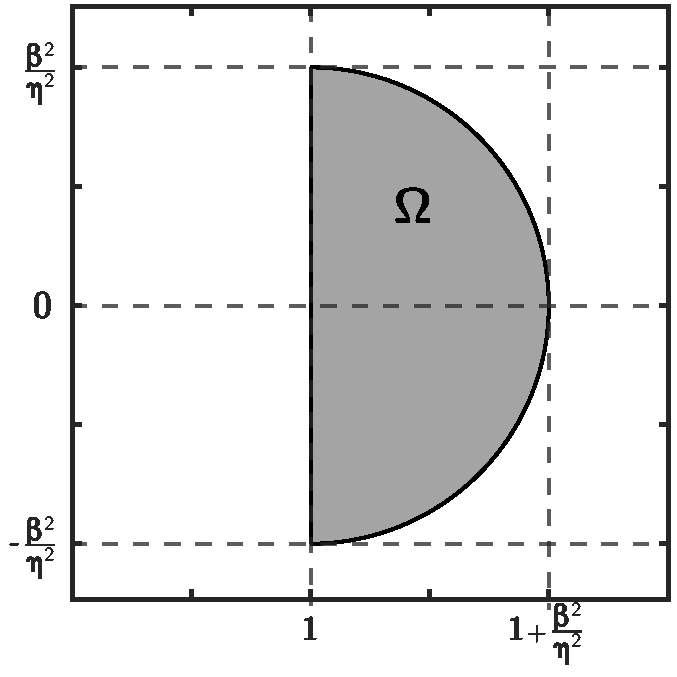
\includegraphics[width = 0.3\textwidth]{./figures/fov.pdf}
\caption{Field-of-values bound for $\mathcal{P}_\eta$ in the complex plane.}
\label{fig:bound}
\end{figure}
\end{theorem}
\begin{proof}
Let $\sigma(B)$ denote the spectrum of operator $B$, $\sigma_{\textnormal{min}}(B)$
and $\sigma_{\textnormal{max}}(B)$ the minimum and maximum eigenvalues, and $\rho(B)$
the spectral radius. Also, define the symmetric/skew-symmetric splitting
$B = B_s + B_k$, where $B_s := (B+B^T)/2$ and $B_k := (B - B^T)/2$, and the numerical
radius as $r(B) = \sup \{ |\lambda| : \lambda \in W(B) \}$. Recall
the following properties of $W(B)$ \cite{gustafson1997numerical,mees1979domains}:
%
\begin{enumerate}
	\item $Bs \leq 0$ in the symmetric negative semi-definite sense
	if and only if $W(B) \leq 0$.

	\item $W(B)\subset [\sigma_{\textnormal{min}}(B_s), \sigma_{\textnormal{max}}(B_s)] \times
	[-\rho(B_k)\mathrm{i}, \rho(B_k)\mathrm{i}]$.

	\item $\sigma(B) \subset W(B)$.

	% <Bv,v> + <v,Bv> > 0 ---> w = B^{-1}v ---> <w, B^{-1}w> + <B^{-1}w,w> > 0
	\item If $B$ is invertible and $B_s \leq 0$ in the symmetric negative semi-definite
	sense, then the symmetric part of $B^{-1}$ is also negative semi-definite.

	\item $r(B) \leq \|B\|_2$.

	\item $W(I + B) = 1 + W(B)$.
\end{enumerate}
%
Note that an exact inverse yields $\mathcal{P}_\eta = I$, with spectrum
and field of values given by $\sigma(\mathcal{P}_S) = W(\mathcal{P}_S) = \{1\}$.
Appealing to \eqref{eq:prec1} and the final property stated above, $W(\mathcal{P}_\eta)
= 1 + \tfrac{\beta^2}{\eta^2}W(E)$, for error term $E := (I - \tfrac{1}{\eta}\widehat{\mathcal{L}})^{-2}$
and real-valued constant $\beta^2/\eta^2 > 0$. Next we will bound $W(E)$ in the complex plane.

Assume that $\eta > 0$ and the symmetric part of $\widehat{\mathcal{L}}$ satisfies
$(\widehat{\mathcal{L}}+\widehat{\mathcal{L}}^T)/2 \leq 0$.
It follows that the real part of eigenvalues of $\widehat{\mathcal{L}}$ are non-positive and,
thus, $(I - \tfrac{1}{\eta}\widehat{\mathcal{L}})$ cannot have a zero eigenvalue and must be
invertible. Furthermore, it also follows that the symmetric part of
$(I - \tfrac{1}{\eta}\widehat{\mathcal{L}})$ is symmetric positive definite and thus
the symmetric part of $(I - \tfrac{1}{\eta}\widehat{\mathcal{L}})^{-2}$ is as well.
This yields a lower bound of zero on the real-axis for $W(E)$, that is,
Re$(W(E)) > 0$.

Now, note that by the assumption $(\widehat{\mathcal{L}}+\widehat{\mathcal{L}}^T)/2 \leq 0$, we have
%
\begin{align}\label{eq:norm1}
\frac{\left\langle (I - \tfrac{1}{\eta}\widehat{\mathcal{L}})\mathbf{x},(I - \tfrac{1}{\eta}\widehat{\mathcal{L}})\mathbf{x}\right\rangle}
	{\langle\mathbf{x},\mathbf{x}\rangle}
& = 1 - \frac{\langle (\widehat{\mathcal{L}} + \widehat{\mathcal{L}}^T )
	\mathbf{x},\mathbf{x}\rangle}{\eta \langle\mathbf{x},\mathbf{x}\rangle} +
	\frac{\langle \tfrac{1}{\eta^2}\widehat{\mathcal{L}}^T\widehat{\mathcal{L}}\mathbf{x},
	\mathbf{x}\rangle}{\langle\mathbf{x},\mathbf{x}\rangle}
\geq 1
\end{align}
%
for all $\mathbf{x}\neq\mathbf{0}$. Then,
%
\begin{align*}
\|(I - \tfrac{1}{\eta}\widehat{\mathcal{L}})^{-2}\| \leq \|(I - \tfrac{1}{\eta}\widehat{\mathcal{L}})^{-1}\|^2
& = \sup_{\mathbf{x}\neq\mathbf{0}}
	\frac{\left\langle (I - \tfrac{1}{\eta}\widehat{\mathcal{L}})^{-1}\mathbf{x},
	(I - \tfrac{1}{\eta}\widehat{\mathcal{L}})^{-1}\mathbf{x}\right\rangle}
	{\langle\mathbf{x},\mathbf{x}\rangle} \\
&\hspace{-10ex}= \sup_{\mathbf{y}\neq\mathbf{0}}
	\frac{\langle\mathbf{y},\mathbf{y}\rangle}{\left\langle (I - \tfrac{1}{\eta}\widehat{\mathcal{L}})\mathbf{y},
	(I - \tfrac{1}{\eta}\widehat{\mathcal{L}})\mathbf{y}\right\rangle}
\leq 1.
\end{align*}
%
This yields a bound on the numerical radius $r(E) = r((I - \tfrac{1}{\eta}\widehat{\mathcal{L}})^{-2})
\leq \|(I - \tfrac{1}{\eta}\widehat{\mathcal{L}})^{-2}\|\leq 1$. Combining with Re$(W(E)) > 0$,
the field of values of the error term, $W(E)$, is contained in the positive half of the
unit circle in the complex plane, which completes the proof.
\end{proof}
%

%
\begin{corollary}[GMRES convergence bounds]\label{cor:gmres}
Let $\pi_k$ denote the set of consistent polynomials of degree $k$. Then the ideal GMRES bound
(an upper bound in operator norm of worst-case convergence) on convergence after $k$ iterations
applied to the preconditioned operator $\mathcal{P}_\eta$ \eqref{eq:prec1} is bounded by
\begin{align*}
\min_{p\in\pi_k} \|p(\mathcal{P}_\eta)\| \leq 2\left(\frac{\beta^2/\eta^2}{2 + \beta^2/\eta^2}\right)^k.
\end{align*}
\end{corollary}
\begin{proof}
For operator $B$, let $\nu(B)$ denote the distance of $W(B)$ from the origin and define
$\cos(\zeta) := \nu(B) / r(B)$. In \cite{liesen2012field}, new convergence
estimates are derived for GMRES based on the field of values. Combining Equations (3.6)
and (3.9) in \cite{liesen2012field} yields a worst-case convergence bound for GMRES
applied to operator $B$ as
%
\begin{align}\label{eq:gmres}
\min_{p\in\pi_k} \|p(B)\| \leq 2\left(\frac{1-\cos\zeta}{1+\cos\zeta}\right)^k.
\end{align}
%
For $B = \mathcal{P}_\eta$, we have $\nu(\mathcal{P}_\eta)= 1$ and
$r(\mathcal{P}_\eta) \leq 1+\beta^2/\eta^2$.
Plugging into \eqref{eq:gmres} completes the proof.\footnote{Note, classical GMRES convergence
results based on $\lambda_{\textnormal{min}}((\mathcal{P}_\eta+\mathcal{P}_\eta^T)/2)$ and
$\lambda_{\textnormal{max}}(\mathcal{P}_\eta^T\mathcal{P}_\eta)$ can also be applied, yielding
the bound $\Big(\tfrac{\beta^2/\eta^2}{1 + \beta^2/\eta^2}\Big)^{k/2}$, $2-4\times$
slower convergence than \Cref{th:fov}.}
\end{proof}
%

%
\begin{corollary}[CG convergence bounds]\label{cor:cg}
Define $\mathcal{Q}_\eta$ as in \eqref{eq:imag1} and $\mathcal{P}_\eta$ as in \eqref{eq:prec1},
and assume $(\eta I - \widehat{\mathcal{L}})$ is SPD. Then, the error $\mathbf{e}_k$ in the
$\mathcal{Q}_\eta$-norm after $k$ iterations of preconditioned CG is bounded by
\begin{align*}
\frac{\|\mathbf{e}_k\|_{\mathcal{Q}_\eta}}{\|\mathbf{e}_0\|_{\mathcal{Q}_\eta}}
	\leq 2\left(\frac{\sqrt{1+\beta^2/\eta^2}-1}{\sqrt{1+\beta^2/\eta^2}+1}\right)^{k}.
\end{align*}
\end{corollary}
\begin{proof}
By assumption, $(\eta I - \widehat{\mathcal{L}})$ is SPD, which implies $\mathcal{Q}_\eta$
and $(\eta I - \widehat{\mathcal{L}})$ are SPD. Then, recall that for preconditioned CG
with preconditioned operator $\mathcal{P}_\eta$, error is bounded via \todo{find reference}
\begin{align}\label{eq:cg_th}
\frac{\|\mathbf{e}_k\|_{A}}{\|\mathbf{e}_0\|_{A}}
	\leq 2\left(\frac{\sqrt{\lambda_{max}(\mathcal{P}_\eta)/\lambda_{min}(\mathcal{P}_\eta)}-1}
	{\sqrt{\lambda_{max}(\mathcal{P}_\eta)/\lambda_{min}(\mathcal{P}_\eta)}+1}\right)^{k},
\end{align}
%
for largest and smallest eigenvalues $\lambda_{max}$ and $\lambda_{min}$, respectively.
Then, recall that eigenvalues of an operator are contained in the field of values, and
from \Cref{th:fov}. This yields $\lambda_{max}(\mathcal{P}_\eta)/\lambda_{min}(\mathcal{P}_\eta)
\leq 1+\beta^2/\eta^2$, and by monotonicity of \eqref{eq:cg_th} in the variable
$(\lambda_{max}(\mathcal{P}_\eta)/\lambda_{min}(\mathcal{P}_\eta))$, this completes
the proof.
\end{proof}
%

\Cref{tab:beta} provides the values of $\eta$, $\beta^2/\eta^2$, and the CG and GMRES
bounds from \Cref{cor:gmres} and \Cref{cor:cg} for Gauss, Radau IIA, and Lobatto IIIC
integration.

%
{
\renewcommand{\tabcolsep}{4pt}
\renewcommand{\arraystretch}{1.15}
\begin{table}[!ht]
  \centering
  \begin{tabular}{| c | c | c | cc | cc | ccc |}  % chktex 44
  \hline
& Stages & 2 & \multicolumn{2}{c}{3} & \multicolumn{2}{|c}{4} & \multicolumn{3}{|c|}{5} \\\hline\hline
\multirow{ 3}{*}{Gauss}
&$\eta$ & 3.0 & 4.64 & 3.68 & 4.21 & 5.79 & 7.29 & 4.65 & 6.70 \\
&$\beta^2/\eta^2$ & 0.33 & 0 & 0.91 & 1.59 & 0.09 & 0 & 2.36 & 0.27 \\
&CG & 0.072 & 0 & 0.160 & 0.234 & 0.022 & 0 & 0.294 & 0.060 \\
&GMRES & 0.143 & 0 & 0.313 & 0.444 & 0.043 & 0 & 0.541 & 0.119  \\\hline
\multirow{ 3}{*}{Radau IIA}
&$\eta$ & 2.0 & 3.64 & 2.68 & 3.21 & 4.79 & 6.29 & 3.66 & 5.70 \\
&$\beta^2/\eta^2$ & 0.50 & 0 & 1.29 & 2.21 & 0.11 & 0 & 3.20 & 0.32	\\
&CG & 0.101 & 0 & 0.205 & 0.283 & 0.025 & 0 & 0.344 & 0.069 \\
&GMRES & 0.2 & 0 & 0.393 & 0.525 & 0.051 & 0 & 0.616 & 0.137 \\\hline
\multirow{ 3}{*}{Lobatto IIIC}
&$\eta$ & 1.0 & 2.63 & 1.69 & 2.22 & 3.78 & 5.28 & 2.66 & 4.70 \\
&$\beta^2/\eta^2$ & 1 & 0 & 2.21 & 3.51 & 0.13 & 0 & 4.88 & 0.38 \\
&CG & 0.172 & 0 & 0.284 & 0.360 & 0.031 & 0 & 0.416 & 0.081 \\
&GMRES & 0.333 & 0 & 0.525 & 0.637 & 0.063 & 0 &  0.709 & 0.161 \\
  \hline
  \end{tabular}
  \caption{$\eta$, $\beta^2/\eta^2$, and the convergence factors in \Cref{cor:gmres}
  and \Cref{cor:cg} for GMRES and CG, respectively (without the leading constants of
  2) for Gauss, Radau IIA, and Lobatto IIIC integration,
  with 2--5 stages. Each column within a given set of stage columns corresponds to a
  conjugate pair of eigenvalues of $A_0^{-1}$. For odd numbers of stages, one eigenvalue
  is real, corresponding to the column where $\beta^2/\eta^2 = 0/\eta^2 = 0$.}\label{tab:beta}
\end{table}
% Gauss
% 2: 1.732050807568877^2/3.000000000000000^2
% 3: 0, 3.508761919567443^2/3.677814645373916^2			(4.644370709252176)
% 4: 5.31483608371350543^2/4.20757879435925566^2, 1.73446825786900750^2/5.79242120564074434^2
% 5: 0, 7.14204584067595280^2/4.64934860636329045^2, 3.48532283236639545^2/6.70391279830706629^2, 		(7.29347719065928652)
% Radau IIA
% 2: 1.414213562373095^2/2^2
% 3: 0, 3.050430199247409^2/2.681082873627745^2	(3.637834252744503)
% 4: 4.77308743327664250^2/3.21280689687153398^2, 1.56747641689520812^2/4.78719310312846602^2
% 5: 0, 6.54373689936007729^2/3.65569432546357226^2, 3.21026560030854989^2/5.70095329867178942^2				(6.28670475172927665)
% Lobatto
% 2: 1
% 3: 0, 2.50873175492488^2/1.687091590520768^2 			(2.625816818958466)
% 4: 4.160391445506932^2/2.220980032989805^2, 1.38017652427285^2/3.779019967010193^2
% 5:
}

% ------------------------------------------------------------------------------------- %
\subsection{Conditioning independent of $\eta$ and $\beta$}\label{sec:solve:gamma}

In the previous section, we considered two applications of $(\eta I -
\widehat{\mathcal{L}})^{-1}$ as a preconditioner for $\mathcal{Q}_\eta$ \eqref{eq:imag1}.
\Cref{th:fov} and the corresponding Corollaries proved that preconditioned
GMRES is guaranteed to converge using such an approach, with bounds on convergence
provided in \Cref{tab:beta}. However, one can note from \Cref{fig:bound} and
\Cref{tab:beta} that convergence depends on values of $\beta$ and $\eta$ and, in
particular, that convergence degrades as the number of stages increase. Ideally,
we would like to observe convergence independent of $\beta$ and $\eta$, analogous
to spatial solvers that achieve convergence independent of spatial mesh and
discretization order. This section is motivated by \cite{exh}, where a similar
algorithm is developed for linear parabolic problems using the real Schur
decomposition, and, for SPD operators, a modified constant $\eta \mapsto
\sqrt{\eta^2+\beta^2}$ is derived, where the preconditioned operator has
condition number $<2$, independent of $\eta$ and $\beta$. In this section,
we derive bounds on the condition number of the preconditioned operator for
preconditioner $(\gamma I - \widehat{\mathcal{L}})^{-2}$, $0 < \gamma\neq \eta$
(\Cref{th:cond}). \Cref{cor:independent} then proves that the constant
%
\begin{align}\label{eq:gam_opt}
\gamma _* := \sqrt{\eta^2+\beta^2}
\end{align}
%
yields a preconditioned operator with condition number $<9$, independent
of $\eta$ and $\beta$.

Consider a similar preconditioner as in
\Cref{sec:solve:inv}, but with some constant $\gamma \mapsto
(\gamma I - \widehat{\mathcal{L}})^{-2}$. The resulting preconditioned
operator takes the form
%
\begin{align}\nonumber
\mathcal{P}_\gamma & =
(\gamma I - \mathcal{L})^{-2}\Big[(nI - \mathcal{L})^2 + \beta^2 I\Big] \\ \nonumber
& = (\gamma I - \mathcal{L})^{-2}\Big[((\eta-\gamma)I + (\gamma I - \mathcal{L}))^2 + \beta^2 I\Big] \\
% & = (\gamma I - \mathcal{L})^{-2}\Big[(\gamma-\eta)^2I - 2(\gamma-\eta)(\gamma I - \mathcal{L}) +
% 	(\gamma I - \mathcal{L})^2 + \beta^2 I\Big] \nonumber\\
& = I - 2(\gamma-\eta)(\gamma I - \mathcal{L})^{-1} + (\beta^2 + (\gamma-\eta)^2)(\gamma I -
	\mathcal{L})^{-2} \nonumber\\
& = I - 2\frac{\gamma-\eta}{\gamma}\left(I - \tfrac{1}{\gamma}\mathcal{L}\right)^{-1} +
	\frac{\beta^2 + (\gamma-\eta)^2}{\gamma^2}
	\left(I - \tfrac{1}{\gamma}\mathcal{L}\right)^{-2}.\label{eq:prec_k}
\end{align}
%
Note that in \eqref{eq:prec_k} we have a quadratic polynomial in
$(I - \tfrac{1}{\gamma}\mathcal{L})^{-1}$. Although this provides
nice structure, the field of values analysis applied in \Cref{sec:solve:inv}
becomes much more complicated due to no necessary relation between
$\langle A\mathbf{x},\mathbf{x}\rangle$ and
$\langle A^2\mathbf{x},\mathbf{x}\rangle$ for general operators $A$. Thus, here
we take a different approach, analyzing the condition number of the preconditioned
operator, $\mathcal{P}_\gamma$, similar to as done for SPD matrices in \cite{exh}.
Although the conditioning does not yield immediate GMRES bounds as the field of values
analysis does (or as conditioning does for bounds on CG convergence), it still
provides a robust measure of the effectiveness and scalability of the
preconditioner.

As a preliminary result, note that working out the roots of the polynomial
in \eqref{eq:prec_k}, it can be expressed in factored form as
%
\begin{align*}
\mathcal{P}_\gamma
	& = \Big[I - \overline{\alpha}\left(I - \tfrac{1}{\gamma}\mathcal{L}\right)^{-1}\Big]
	\Big[I - \alpha\left(I - \tfrac{1}{\gamma}\mathcal{L}\right)^{-1}\Big],
\end{align*}
%
where
%
\begin{align}\label{eq:alpha}
\alpha, \overline{\alpha} & := 1 - \frac{\eta}{\gamma} \pm \mathrm{i}\beta,
\end{align}
%
and
%
\begin{align}\label{eq:alpha_eq}
\alpha + \overline{\alpha} = 2(1 - \tfrac{\eta}{\gamma}), \hspace{5ex}
\alpha\overline{\alpha} = \tfrac{\beta^2 + (\gamma-\eta)^2}{\gamma^2}.
\end{align}
%
Moving forward we will limit ourselves to considering $\eta \leq \gamma \leq \
\tfrac{\eta^2+\beta^2}{\eta}$, which limits to the natural case of $\gamma = \eta$
as $\beta \to 0$. Similar analysis can be performed for $\gamma$ outside of
this range, but the derivations are different and there does not appear to
be any good reason to use $\gamma$ outside of this range (for some detail,s
see discussion following \Cref{th:cond}, and in \cite{exh} for SPD operators).

%
\begin{theorem}[Conditioning of preconditioned operator]\label{th:cond}
Suppose Assumptions \ref{ass:eig} and \ref{ass:fov} hold, that is, $\eta > 0$
and $W(\mathcal{L}) \leq 0$ \eqref{eq:fov}. Let $\eta \leq \gamma \leq \
\tfrac{\eta^2+\beta^2}{\eta}$ for $\gamma\in\mathbb{R}$ and let
$\mathcal{P}_\gamma$ denote the preconditioned operator, where $((\eta + i\beta)I -
\widehat{\mathcal{L}})((\eta - i\beta)I - \widehat{\mathcal{L}})$ is
preconditioned with $(\gamma I - \widehat{\mathcal{L}})^{-2}$. Then,
\begin{align}\label{eq:cond1}
\textnormal{cond}(\mathcal{P}_\gamma) \leq (1 + \alpha\overline{\alpha})
		\left(1 + \frac{\alpha\overline{\alpha}}{(1 - \alpha)(1 - \overline{\alpha})}\right)
	% \begin{cases}
	% \frac{1 + \alpha\overline{\alpha}} {(1 - \alpha)(1 - \overline{\alpha})}
	% 	& \eta\gamma \geq \eta^2+\beta^2, \\
	% (1 + \alpha\overline{\alpha})
	% 	\left(1 + \frac{\alpha\overline{\alpha}}{(1 - \alpha)(1 - \overline{\alpha})}\right)
	% 	& \eta\gamma < \eta^2+\beta^2,
	% \end{cases}
\end{align}
with $\alpha$ and $\overline{\alpha}$ defined as in \eqref{eq:alpha}.
\end{theorem}
\begin{proof}
The proof proceeds by using the factored form of $\mathcal{P}_\gamma$ \eqref{eq:prec_k},
to derive an upper bound on $\|\mathcal{P}_\gamma\|$ and $\|\mathcal{P}_\gamma^{-1}\|$,
which immediately yields a bound on
%
\begin{align}\label{eq:cond0}
\textnormal{cond}(\mathcal{P}_\gamma) = \|\mathcal{P}_\gamma\|\|\mathcal{P}_\gamma^{-1}\|.
\end{align}
%
Note that following from the discussion in \Cref{sec:solve:inv} and \Cref{th:fov},
for real $\gamma>0$, $W\left[(I - \tfrac{1}{\gamma}\mathcal{L})^{-1}\right]$ and
$W\left[(I - \tfrac{1}{\gamma}\mathcal{L})^{-2}\right]$ are contained in
the positive half unit circle, and $\|(I - \tfrac{1}{\gamma}\mathcal{L})^{-1}\| \leq 1$
(see proof of \Cref{th:fov}).

We start with $\|\mathcal{P}_\gamma\|$, where
%
\begin{align}\label{eq:CS}
\|\mathcal{P}_\gamma\| & \leq
	\Big\|I - \overline{\alpha}\left(I - \tfrac{1}{\gamma}\mathcal{L}\right)^{-1}\Big\|
	\Big\|I - \alpha\left(I - \tfrac{1}{\gamma}\mathcal{L}\right)^{-1}\Big\|.
\end{align}
%
Recall that $W\left[(I - \tfrac{1}{\gamma}\mathcal{L})^{-1}\right] \geq 0$
and $\|(I - \tfrac{1}{\gamma}\mathcal{L})^{-1}\| \leq 1$. Using the
assumption $\gamma \geq \eta \implies(\alpha+\overline{\alpha}) \geq 0$,
we can expand the norm squared in inner-product form, yielding
%
\begin{align*}
&\hspace{-5ex}
\Big\|I - \overline{\alpha}\left(I - \tfrac{1}{\gamma}\mathcal{L}\right)^{-1}\Big\|^2 \\
	& = 1 + \max_{\mathbf{x}\neq\mathbf{0}} \left( \alpha\overline{\alpha}
		\frac{\left\|\left(I - \tfrac{1}{\gamma}\mathcal{L}\right)^{-1}\mathbf{x}\right\|^2
		}{\|\mathbf{x}\|^2}
	- (\alpha + \overline{\alpha})\frac{\textnormal{Re}\left(\left\langle\left(I -
		\tfrac{1}{\gamma}\mathcal{L}\right)^{-1}\mathbf{x}, \mathbf{x}\right\rangle\right)}
		{\|\mathbf{x}\|^2}\right) \\
& \leq 1 + \alpha\overline{\alpha}\left\|\left(I - \tfrac{1}{\gamma}\mathcal{L}\right)^{-1}\right\|^2 \\
& \leq 1 + \alpha\overline{\alpha}.
\end{align*}
%
Note that the above derivation is identical for $\alpha$ and $\overline{\alpha}$,
which yields
%
\begin{align} \label{eq:upper_alpha}
\|\mathcal{P}_\gamma\| & \leq 1 + \alpha\overline{\alpha}.
\end{align}
%

To bound $\|\mathcal{P}_\gamma^{-1}\|$, we use an analogous approach as above
\eqref{eq:CS}, developing bounds on the two polynomial factors separately.
First, note that
%
\begin{align}\nonumber
\left[I - \alpha\left(I - \tfrac{1}{\gamma}\mathcal{L}\right)^{-1}\right]^{-1}
	& = \left(I - \tfrac{1}{\gamma}\mathcal{L}\right)
		\left[(1-\alpha)I - \tfrac{1}{\gamma}\mathcal{L}\right]^{-1} \nonumber\\
& = \left[\alpha I + ((1-\alpha)I - \tfrac{1}{\gamma}\mathcal{L})\right]
		\left[(1-\alpha)I - \tfrac{1}{\gamma}\mathcal{L}\right]^{-1} \nonumber\\
& = I + \alpha \left[(1-\alpha)I - \tfrac{1}{\gamma}\mathcal{L}\right]^{-1} \nonumber\\
& = I + \frac{\alpha}{1-\alpha} \left(I - \tfrac{1}{\gamma(1-\alpha)}\mathcal{L}\right)^{-1}.
	\label{eq:inv_factor}
\end{align}
%
For condensed notation, let $c_\alpha := \tfrac{\alpha}{1-\alpha}$, and note that
%
\begin{align*}
c_\alpha+\overline{c_\alpha} & = \frac{\alpha + \overline{\alpha} - 2\alpha\overline{\alpha}}
	{1 + \alpha\overline{\alpha} - (\alpha + \overline{\alpha})}
= \frac{2\eta\gamma - 2(\eta^2+\beta^2)}{\eta^2+\beta^2},
\end{align*}
%
which is $\leq 0$ when $\eta\gamma \leq (\eta^2+\beta^2)$ and $>0$ otherwise.

Expanding the squared norm of \eqref{eq:inv_factor} in inner-product form, we have
%
{\small
\begin{align}\label{eq:pinv0}
& \hspace{-5ex}
1 + \max_{\mathbf{x}\neq\mathbf{0}} \left[ (c_\alpha+\overline{c_\alpha})
	\frac{\textnormal{Re}\left(\left\langle (I - \tfrac{1}{\gamma(1-\alpha)}\mathcal{L})^{-1}\mathbf{x},
		\mathbf{x}\right\rangle\right)}{\|\mathbf{x}\|^2} +
	c_\alpha\overline{c_\alpha}
	\frac{\left\|(I - \tfrac{1}{\gamma(1-\alpha)}\mathcal{L})^{-1}\mathbf{x}\right\|^2}
		{\|\mathbf{x}\|^2} \right].
\end{align}
}
%
Bounding the norm term in \eqref{eq:pinv0} requires care because $\alpha$ is
complex. Note that the norm is the maximum singular value, which is equivalent to one
over the minimum nonzero singular value of the inverse. The squared minimum nonzero
singular value of the inverse of $(I - \tfrac{1}{\gamma(1-\alpha)}\mathcal{L})^{-1}$
is given by
%
\begin{align*}
&\hspace{-5ex}
\min_{\mathbf{x}\neq\mathbf{0}} \frac{\left\|\left(I - \tfrac{1}{\gamma(1-\alpha)}
	\mathcal{L}\right)\mathbf{x}\right\|^2}{\|\mathbf{x}\|^2} \\
& = 1 + \min_{\mathbf{x}\neq\mathbf{0}} \left[ \frac{1}{|\gamma(1-\alpha)|^2}
	\frac{\left\|\mathcal{L}\mathbf{x}\right\|^2}{\|\mathbf{x}\|^2}
	- \left(\frac{1}{\gamma(1-\alpha)} + \frac{1}{{\gamma}(1-\overline{\alpha})}\right)
	\frac{\textnormal{Re}\left(\left\langle\mathcal{L}\mathbf{x},\mathbf{x}\right\rangle\right)}
		{\|\mathbf{x}\|^2}\right].
\end{align*}
%
Noting that Re$\left(\langle\mathcal{L}\mathbf{x},\mathbf{x}\rangle\right) \leq 0$,
$\gamma \geq \eta > 0$, and Re$(1-\alpha) \geq 0$, it follows that the squared minimum
singular value above is $\geq 1$, which implies $\|(I - \tfrac{1}{\gamma(1-\alpha)}
\mathcal{L})^{-1}\| \leq 1$.

% ------> Old extra derivation for \gamma larger than currently considered
% ------------------------------------------------------------------------
% Plugging into \eqref{eq:pinv1} and noting
% that an identical derivation and result holds for $\overline{\alpha}$, we have
% for $(c_\alpha+\overline{c_\alpha}) \geq 0$,
% %
% \begin{align}\nonumber
% \|\mathcal{P}_\gamma^{-1}\| & \leq
% 	\Big\|\Big(I - \overline{\alpha}\left(I - \tfrac{1}{\gamma}\mathcal{L}\right)^{-1}\Big)^{-1}\Big\|
% 	\Big\|\Big(I - \alpha\left(I - \tfrac{1}{\gamma}\mathcal{L}\right)^{-1}\Big)^{-1}\Big\| \\
% & \leq \left(1 + \frac{\alpha}{1-\alpha}\right)
% 	\left(1 + \frac{\overline{\alpha}}{1-\overline{\alpha}}\right) \nonumber\\
% & = \frac{1}{(1 - \alpha)(1 - \overline{\alpha})}. \label{eq:lower_alpha1}
% \end{align}
% %

Returning to \eqref{eq:pinv0}, consider the inner-product term with leading
constant $(c_\alpha+\overline{c_\alpha}) \leq 0$. Note that letting
$\mathbf{x}:= (I - \tfrac{1}{\gamma(1-\alpha)}\mathcal{L})\mathbf{y}$,
we have
%
\begin{align*}
\frac{\left\langle (I - \tfrac{1}{\gamma(1-\alpha)}\mathcal{L})^{-1}\mathbf{x},
		\mathbf{x}\right\rangle}{\|\mathbf{x}\|^2}
& = \frac{\left\langle \mathbf{y}, (I - \tfrac{1}{\gamma(1-\alpha)}\mathcal{L})\mathbf{y}
	\right\rangle}{\|(I - \tfrac{1}{\gamma(1-\alpha)}\mathcal{L})\mathbf{y}\|^2}
= \frac{\|\mathbf{y}\|^2 - \frac{1}{\gamma (1 - \overline{\alpha})}
	\left\langle \mathbf{y},\mathcal{L}\mathbf{y} \right\rangle}
	{\|(I - \tfrac{1}{\gamma(1-\alpha)}\mathcal{L})\mathbf{y}\|^2}.
\end{align*}
%
By assumption, Re$\left(\langle \mathbf{y},\mathcal{L}\mathbf{y}\rangle\right) \leq 0$,
while $\gamma\geq 0$ and Re$(1-\alpha) \geq 0$. It follows that
%
\begin{align*}
\textnormal{Re}\left(\frac{\left\langle (I - \tfrac{1}{\gamma(1-\alpha)}\mathcal{L})^{-1}\mathbf{x},
	\mathbf{x}\right\rangle}{\|\mathbf{x}\|^2}\right) \geq 0.
\end{align*}
%
Thus in \eqref{eq:pinv0} because $(c_\alpha+\overline{c_\alpha}) \leq 0$, we can drop
the corresponding term for an upper bound of
%
\begin{align*}
\left\|\left[I - \alpha\left(I - \tfrac{1}{\gamma}\mathcal{L}\right)^{-1}\right]^{-1}\right\|^2
	& \leq 1 + c_\alpha\overline{c_\alpha}
		\left\|(I - \tfrac{1}{\gamma(1-\alpha)}\mathcal{L})^{-1}\right\|^2 \\
& \leq 1 + c_\alpha\overline{c_\alpha} \\
& = 1 + \frac{\alpha\overline{\alpha}}{(1 - \alpha)(1 - \overline{\alpha})}.
\end{align*}
%
Again noting that analogous derivations holds for $\overline{\alpha}$ with
identical bounds, we have for $(c_\alpha+\overline{c_\alpha}) < 0$,
%
\begin{align}
\|\mathcal{P}_\gamma^{-1}\| & \leq 1 +
	\frac{\alpha\overline{\alpha}}{(1 - \alpha)(1 - \overline{\alpha})}. \label{eq:lower_alpha2}
\end{align}
%

Combining \eqref{eq:cond0}, \eqref{eq:upper_alpha},
and \eqref{eq:lower_alpha2} completes the proof.
\end{proof}
%

In \cite{exh}, similar analysis is done under the assumption
that $-\mathcal{L}$ is SPD, in which case the conditioning can be derived based on
eigenvalues. There, they effectively derive the conditioning of the preconditioned
operator for $\gamma = \eta$ to be cond$(\mathcal{P}_\eta) = 1 + \tfrac{\beta^2}{\eta^2}$
(using notation of this paper, as the spectrum of $(I - \tfrac{1}{\eta}\mathcal{L})^{-1}
\mapsto [0,1]$, as would likely happen with refinement of a parabolic problem,
the result in \cite{exh} is exact).
If we let $\gamma = \eta$, from \eqref{eq:alpha_eq} we have
$\alpha+\overline{\alpha} = 0$, $\alpha\overline{\alpha} =
\frac{\beta^2}{\eta^2}$, and \Cref{th:cond} yields
%
\begin{align}\label{eq:cond_eta}
\textnormal{cond}(\mathcal{P}_{\gamma = \eta}) \leq 1 + 2\frac{\beta^2}{\eta^2}.
\end{align}
%
In particular, this indicates that \Cref{th:cond} is fairly tight (it is unclear
if the additional factor of 2 in \eqref{eq:cond_eta} is necessary for non-SPD
operators, or a flaw in the line of proof).
Considering the upper limit on $\gamma$ in \Cref{th:cond}, $\gamma \mapsto
\tfrac{\eta^2+\beta^2}{\eta}$, we have a bound
%
\begin{align}\label{eq:cond_upper}
\textnormal{cond}\left(\mathcal{P}_{\gamma = \frac{\eta^2+\beta^2}{\eta}}\right) \leq
	\left(1 + \frac{\beta^2}{\eta^2}\right) \left(1 + \frac{\beta^2}{\beta^2 + \eta^2}\right).
\end{align}
%
Note, in both \eqref{eq:cond_eta} and \eqref{eq:cond_upper} we see a dependence
on $\eta$ and $\beta$.

In \cite{exh}, they also derive a constant to minimize certain bounds on condition
number for SPD matrices, $\gamma _* := \sqrt{\eta^2+\beta^2}$ \eqref{eq:gam_opt}
(also the exact minimizer as the spectrum of $(I - \tfrac{1}{\eta}\mathcal{L})^{-1}
\mapsto [0,1]$). Considering $\gamma_*$ here, \eqref{eq:alpha_eq} yields
$\alpha+\overline{\alpha} = \alpha\overline{\alpha} =
2 - 2\frac{\eta}{\sqrt{\eta^2+\beta^2}}$, and \Cref{th:cond} yields the bound
%
\begin{align}\label{eq:cond_opt}
\textnormal{cond}(\mathcal{P}_{\gamma_*})
	\leq \left(3 - 2\frac{\eta}{\sqrt{\eta^2+\beta^2}}\right)^2.
\end{align}
%
Noting that $\textnormal{cond}(\mathcal{P}_{\gamma_*}) < 9$ for all $\eta>0,
\beta\geq 0$, we have the following corollary.

%
\begin{corollary}[Conditioning independent of $\eta$ \& $\beta$]\label{cor:independent}
\textnormal{ }
Preconditioning $\mathcal{Q}_\eta$ \eqref{eq:imag1} with
$(\gamma_* I - \widehat{\mathcal{L}})^{-2}$, for $\gamma_* = \sqrt{\eta^2+\beta^2}$
yields a preconditioned operator $\mathcal{P}_{\gamma_*}$ such that
$\textnormal{cond}(\mathcal{P}_{\gamma_*}) < 9$,
independent of $\eta$ and $\beta$.
\end{corollary}
%
It is worth pointing out that as $\beta \to 0$, $\gamma \to \eta$
in all three of the above cases, and (as expected) \eqref{eq:cond_eta},
\eqref{eq:cond_upper}, and \eqref{eq:cond_opt} all $\to 1$. \Cref{tab:cond}
provides condition number bounds for Gauss, Radau IIA, and Lobatto IIIC
Runge-Kutta methods.
Finally, although the difference in conditioning between \eqref{eq:cond_eta}
and \eqref{eq:cond_opt} does not appear large for reasonable values of
$\eta$ and $\beta$, examples in \Cref{sec:numerics:dg} demonstrate up to
a $5.8\times$ reduction in iteration count achieved by using $\gamma_*$
instead of $\eta$.

%
{
\renewcommand{\tabcolsep}{4pt}
\renewcommand{\arraystretch}{1.15}
\begin{table}[!ht]
  \centering
  \begin{tabular}{| c | c | cc | cc | ccc |}  % chktex 44
  \hline
Stages & 2 & \multicolumn{2}{c}{3} & \multicolumn{2}{|c}{4} & \multicolumn{3}{|c|}{5} \\\hline\hline
Gauss & 1.61 & 1 & 2.41 & 1.17 & 3.09 & 1 & 1.50 & 3.64 \\
Radau IIA & 1.87 & 1 & 2.82 & 1.21 & 3.55 & 1 & 1.58 & 4.10 \\
Lobatto IIIC & 2.51 & 1 & 3.55 & 1.26 & 4.24 & 1 & 1.69 & 4.73  \\\hline
  \end{tabular}
  \caption{Condition number bounds using constant $\gamma=\gamma_*$ \eqref{eq:cond_opt}
  for preconditioned operators $\mathcal{P}_{\gamma_*}$ arising in Gauss, Radau IIA, and
  Lobatto IIIC integration, with 2--5 stages. Each column within a given set of stage columns corresponds to a conjugate pair of eigenvalues of $A_0^{-1}$. For odd numbers of stages,
  one eigenvalue is real, corresponding to the column with conditioning 1.}\label{tab:cond}
\end{table}
}


%
\begin{remark}[``Optimal'' $\gamma$]
A natural question is what is the optimal $\gamma$ in general?
Let $f(\gamma)$ denote the upper bound from \Cref{th:cond} \eqref{eq:cond1}.
Some algebra shows that
%
\begin{align*}
f'(\gamma) &= \frac{4\gamma^4 - 6\eta\gamma^3 + 4\eta(\eta^2+\beta^2)\gamma -
	2(\eta^2+\beta^2)^2}{(\eta^2+\beta^2)\gamma^3}.
\end{align*}
%
For $\beta > 0$,
%
\begin{align*}
f'(\eta) & = -\frac{2\beta^4}{\eta^3(\eta^2+\beta^2)} < 0,
\hspace{5ex}
f'(\gamma_*) = \frac{2(\sqrt{\eta^2+\beta^2} - \eta)}{\eta^2+\beta^2} > 0.
% f'\left(\tfrac{\eta^2+\beta^2}{\eta}\right) & = 2\beta^2 + \frac{\beta^2}{\eta^2+\beta^2} > 0, \\
\end{align*}
%
Thus there exists a critical point $\gamma \in(\eta,\gamma_*)$, and it is
likely not advantageous to choose $\gamma > \gamma_*$. The equation
for the root is a quartic polynomial and is not examined analytically here,
however, depending on $\eta$ and $\beta$, testing on realistic values suggests
the sign change (and, thus, root) is likely between $0.8\gamma_* - 0.9\gamma_*$,
indicating $\gamma_*$ is indeed a good approximation to the optimal $\gamma$ with
respect to \eqref{eq:cond1}.
% Moreover, the analysis from \cite{exh} proves that $\gamma_*$ \eqref{eq:gam_opt}
% \textit{is} optimal for SPD operators, and we prove $\gamma_*$ also provides
% very good preconditioning independent of the number of stages/order of integration
% in the more general setting (\Cref{cor:independent}).
\end{remark}
%



% ------------------------------------------------------------------------------------- %
% ------------------------------------------------------------------------------------- %
\subsection{Preconditioning in practice}


% ------------------------------------------------------------------------------------- %
\subsubsection{Choosing $\gamma$}

Theory from \Cref{sec:solve:gamma} indicates that for $\beta\leq \eta$, conditioning
independent of $\eta$ and $\beta$ can be obtained by preconditioning with
$(\eta I - \widehat{\mathcal{L}})^{-1}$. However, for $\beta > \eta$, conditioning
independent of these constants likely requires a different constant $\eta\mapsto\gamma$,
with one such option being $\gamma_* = \sqrt{\eta^2+\beta^2}$ \eqref{eq:gam_opt}.
In practice, we have found it simplest to always precondition with
$(\gamma_* I - \widehat{\mathcal{L}})^{-1}$, regardless of $\eta$ and $\beta$.
Although the modified constant is not necessary for $\beta \leq \eta$ (and,
interestingly, also sometimes not necessary for $\beta > \eta$ in practice),
we have observed \textit{no} cases where convergence is worse when using $\gamma_*$
instead of $\eta$, while other situations where $\gamma_*$ has resulted in a $5.8\times$
speedup over $\eta$. Moreover, from a preconditioning perspective, $\gamma_* > \eta$
can be seen as larger identity perturbation to $\widehat{\mathcal{L}}$, making the
resulting operator better conditioned and, thus, potentially more amenable to
constructing effective preconditioners.

% ------------------------------------------------------------------------------------- %
\subsubsection{Mass matrices}

Recall in the finite element context where mass matrices are involved, we defined
$\widehat{\mathcal{L}} := \delta t M^{-1}\mathcal{L}$. For a given conjugate pair
of eigenvalues, the quadratic polynomial \eqref{eq:imag1} can be expressed as
%
\begin{align}\label{eq:scaleM}
\mathcal{Q}_\eta = M^{-1}((\eta + i\beta)M - \delta t{\mathcal{L}})M^{-1}((\eta - i\beta)M -
	\delta t\widehat{\mathcal{L}}).
\end{align}
%
In this context, it is best to first scale both sides of the linear system by $M$.
This halves the number of times $M^{-1}$ must applied for each Krylov iteration,
and if $M$ and $\mathcal{L}$ are Hermitian, the resulting quadratic system is SPD
and can be solved using preconditioned conjugate gradient or MINRES, preconditioned
with one application of a preconditioner, the action of $M$, and a second application
of the preconditioner.

% ------------------------------------------------------------------------------------- %
\subsubsection{Inexact preconditioning}
\label{sec:inexact-precond}

In practice, fully converging $(\eta I - \widehat{\mathcal{L}})^{-1}$ as a preconditioner
is not desirable --  even if a Krylov method converges rapidly, if each iteration requires
a full linear solve, the resulting method remains too expensive to be competitive in practice.
Here, we propose
applying a Krylov method to $\mathcal{Q}_\eta:=(\eta^2+\beta^2)I - 2\eta\widehat{\mathcal{L}} +
\widehat{\mathcal{L}}^2$ by computing the operator's action (that is, not fully constructing
it), and preconditioning each Krylov iteration with \textit{two} applications of a sparse
parallel preconditioner for $(\eta I - \widehat{\mathcal{L}})$, approximating the action
of $(\eta I - \widehat{\mathcal{L}})^{-2}$.

To motive this heuristically, suppose $(\eta I - \widehat{\mathcal{L}}) = B + N$,
where $B^{-1}$ corresponds to the action of a preconditioner and $N$ the error
term that is not captured. For a good preconditioner, we expect
$B^{-1}(\eta I - \widehat{\mathcal{L}}) = I+B^{-1}N$ to be
well-conditioned and, thus, $B^{-1}N$ to be small in some sense. Then,
%
\begin{align}\nonumber
B^{-2}\mathcal{Q}_\eta & = I + \beta^2B^{-2} + \left(B^{-2}NB + B^{-1}N + B^{-2}N^{-2}\right)\label{eq:approx}.
\end{align}
%
In addition to wanting $N$ to be small, it is also important that the error terms
$B^{-2}NB + B^{-1}N + B^{-2}N^{-2}$ are generally positive in a field of values sense.
If these terms are large and positive in a field of values sense, the outer Krylov
iteration applied to $B^{-2}\mathcal{Q}_\eta$ can correct for these modes. However,
if error terms $B^{-2}NB + B^{-1}N + B^{-2}N^{-2}$ in \eqref{eq:approx} have
negative components, the field of values of the preconditioned operator is shifted
towards the origin, wherein Krylov acceleration is of progressively less use.

Thus, theory developed in \Cref{sec:solve:prec} guarantees that the proposed algorithm
will have robust and fairly rapid convergence under reasonable assumptions if each
linear system is inverted exactly. Approximate inverses prove to be much faster in
practice, but \textit{it is important that the underlying preconditioner provides a good
inverse approximation}. Fortunately, for difficult problems with only okay preconditioners,
it is straightforward to apply either multiple inner fixed-point iterations or an
inner Krylov iteration (wrapped with a flexible outer Krylov method
\cite{notay2000flexible,saad1993flexible}) to ensure robust (outer) iterations, analogous
to techniques used in block preconditioning. In \Cref{sec:numerics:dg:diff}, a
numerical example is shown where the proposed method diverges using a single inner
fixed-point iteration as a preconditioner for $(\eta I - \widehat{\mathcal{L}})$, but
three (or more) inner fixed-point iterations yields fast, scalable convergence.

% ------------------------------------------------------------------------------------- %
% ------------------------------------------------------------------------------------- %
% ------------------------------------------------------------------------------------- %
\begin{comment}
\section{Implementation details:  The time-independent case}
The basic idea is that we need to do the update
\begin{align} \label{eq:RK_update}
\bm{u}_{n+1}  = \bm{u}_n + \delta t \mdet({\cal M}_s)^{-1} \big( \bm{b}_0^\top A^{-1}_0 \otimes I \big) \madj({\cal M}_s) \bm{f},
\end{align}
where we have
\begin{itemize}
\item $m \in \mathbb{N}$: The dimension of the spatial problem

\item $\bm{f} = (\bm{f}_1, \ldots, \bm{f}_s)^\top$, with $\bm{f}_j \in \mathbb{R}^m$

\item $\tilde{\bm{b}}^\top_0 \coloneqq \bm{b}^\top_0 A^{-1}_0 \in \mathbb{R}^{1 \times s}$ (this is a row vector, not that this distinction really matters)
\end{itemize}

Now we break \eqref{eq:RK_update} into two steps:
\begin{enumerate}
\item{Step 1:}\label{it:update_step1}Compute
\begin{align} \label{eq:step1}
\bm{z} = \big( \hat{\bm{b}}^\top_0 \otimes I \big) \madj ({\cal M}_s) \bm{f} \in \mathbb{R}^m
\end{align}

\item{Step 2:}\label{it:update_step2} Solve
\begin{align} \label{eq:step2}
\mdet( {\cal M}_s ) \bm{y} = \bm{z},
\end{align}
then update per \eqref{eq:RK_update}, $\bm{u}_{n+1} = \bm{u}_n + \delta t \bm{y}$
\end{enumerate}


\subsection{On Step \ref{it:update_step1}}

The adjugate of ${\cal M}_s$ is a matrix defined over degree  $s-1$ polynomials in ${\cal L} \in \mathbb{R}^{m \times m}$. More specifically, we write it as
\begin{align}
\madj ({\cal M}_s) =
\begin{bmatrix}
Q_{11}({\cal L}) & \cdots & Q_{1s}({\cal L}) \\
\vdots & & \vdots \\
Q_{s1}({\cal L}) & \cdots & Q_{ss}({\cal L})
\end{bmatrix}
\in \mathbb{R}^{ms \times ms},
\quad
Q_{ij}({\cal L}) = \sum \limits_{k = 0}^{s-1} \hat{q}_{ijk} {\cal L}^k \in \mathbb{R}^{m \times m}.
\end{align}

Now, the Kronecker product appearing in front of this matrix simply takes inner products over its columns to give a block rectangular matrix whose elements are therefore polynomials in ${\cal L}$ of degree $s-1$:
\begin{align}
\big( \bm{b}_0^\top A^{-1}_0 \otimes I \big) \madj({\cal M}_s)
=
\begin{bmatrix}
X_{1}({\cal L}), \, \cdots, \, X_{s}({\cal L})
\end{bmatrix},
\end{align}
where
\begin{align}
X_{j}({\cal L}) = \sum \limits_{k = 0}^{s-1} \hat{x}_{j k} {\cal L}^k \in \mathbb{R}^{m \times m},
\quad
\hat{x}_{j k} = \sum \limits_{\ell = 1}^s \big( \tilde{\bm{b}}_0^\top \big)_{\ell} \hat{q}_{\ell j k}.
\end{align}
And, so, finally, the vector in \eqref{eq:step1} can be written as the sum
\begin{align} \label{eq:z_sum}
\bm{z} = \sum \limits_{i = 1}^s X_i({\cal L}) \bm{f}_i.
\end{align}
The main task here is going to be computing the action of the degree $s-1$ polynomials $X_i({\cal L})$ of the components of $\bm{f}$; note that we can  easily compute the sets of coefficients $\{ x_{jk} \}_{(j,k)=(1,0)}^{(s,s-1)}$. I think the most efficient way to compute the action of this polynomial is with a Horner-like scheme which is a well-known technique for evaluating scalar polynomials (see \url{https://en.wikipedia.org/wiki/Horner\%27s_method}). Basically, we can compute the action of the $n$th degree polynomial $P_n({\cal L})$ on a vector using: $n$ \texttt{MATVECs} with ${\cal L}$, $n+1$ \texttt{AXPYs} ($\bm{x} \gets \alpha \bm{y} + \beta \bm{z}$), $n$ \texttt{copies} ($n$ lots of copying values from one vector to another, $n \times [\bm{x} \gets \bm{y}]$), and one intermediate/temporary vector. So the main cost in computing \eqref{eq:z_sum} is $s(s-1)$ \texttt{MATVECs} with ${\cal L}$.
\end{comment}

% ------------------------------------------------------------------------------------- %
% ------------------------------------------------------------------------------------- %
% ------------------------------------------------------------------------------------- %
\section{Numerical results}\label{sec:numerics}

% ------------------------------------------------------------------------------------- %
% ------------------------------------------------------------------------------------- %
\subsection{Finite-difference advection-diffusion}\label{sec:numerics:fd}

In this section, we consider a constant-coefficient advection-diffusion problem
discretized in space with high-order finite-differences. An exact solution to
this problem is used to demonstrate the high-order accuracy of the IRK methods,
and the robustness of the algorithms developed in the previous section with
respect to mesh resolution. Specifically, we solve the PDE
%
\begin{align}
\label{eq:FD_ex} u_t + 0.85 u_x + u_y = 0.3 u_{xx} + 0.25 u_{yy} + s(x,y,t),
\quad (x,y,t) \in (-1,1)^2 \times (0,2],
\end{align}
%
on a periodic spatial domain. The source term $s(x,y,t)$ is chosen such that
the solution of the PDE is
$u(x,y,t)=\sin^4(\pi/2[x-1-0.85t]) \sin^4(\pi/2 [y-1-t]) \exp(-[0.3+0.25]t)$.

We consider tests using IRK methods of orders three, four, seven, and eight. The
3rd- and 4th-order IRK methods are paired with 4th-order
central-finite-differences in space, and the 7th- and 8th-order methods with
8th-order central-finite-differences in space. In all cases, a time-step of
$\delta t = 2 h$ is used, with $h$ denoting the spatial mesh size. Due to the
diffusive, but non-SPD nature of the spatial discretization, we apply GMRES(30)
preconditioned by a classical AMG method in the \textit{hypre} library
\cite{Falgout:2002vu}. Specifically, we
use classical interpolation (type 0), Falgout coarsening (type 6) with a strength
tolerance $\theta_C = 0.25$, zero levels of aggressive coarsening, and
$L_1$-Gauss--Seidel relaxation (type 8), with an absolute and relative stopping
tolerance of $10^{-13}$. A single iteration of AMG is applied to approximate
$(\gamma_* I - \delta t {\cal L})^{-1}$.

In Fig. \ref{fig:FD_ex}, discretization errors are shown for different IRK
methods, alongside the average number of AMG iterations needed per time step.
The expected asymptotic convergence rates (black dashed lines in the left panel)
are observed for all discretizations.\footnote{An exception here is A--SDIRK(4),
which appears to be converging with a rate closer to three than four; however,
further decreasing $\delta t$ (not shown here) confirms 4th-order convergence
is achieved eventually.}

\begin{figure}[!htb]
%\begin{figure}[H]
\centerline{
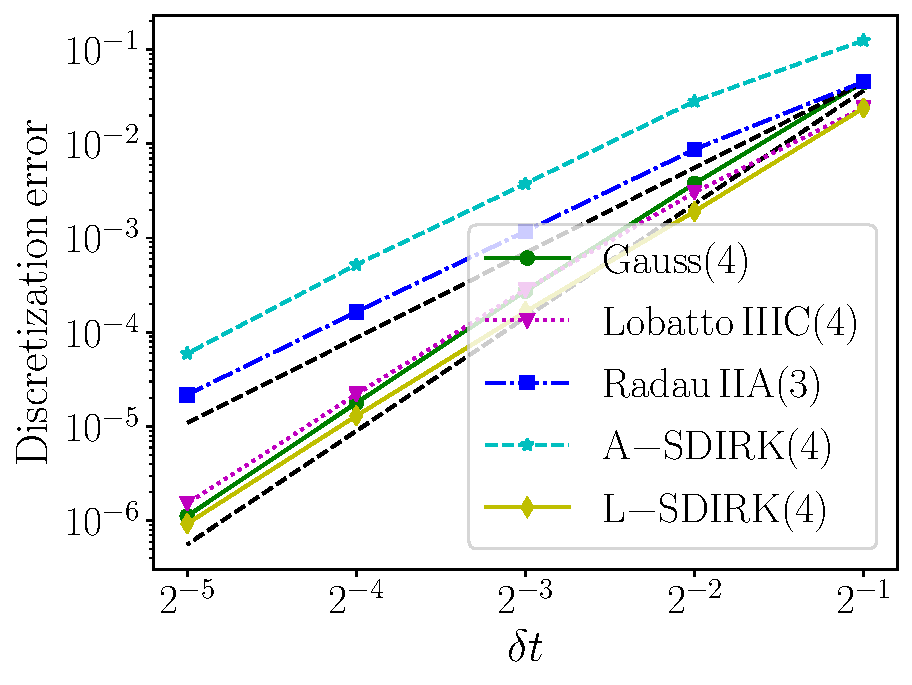
\includegraphics[width = 0.475\textwidth]{figures/FD_ex/errors_iters_14_34_23_-14_4_d2_ex1.pdf}
\quad
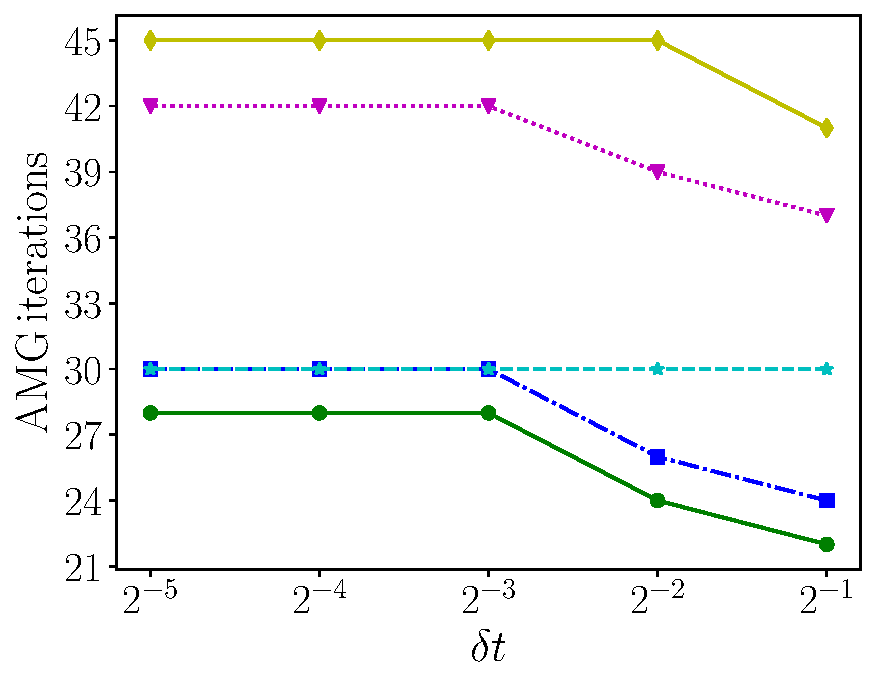
\includegraphics[width = 0.475\textwidth]{figures/FD_ex/amg_iters_14_34_23_-14_4_d2_ex1.pdf}
}
\centerline{
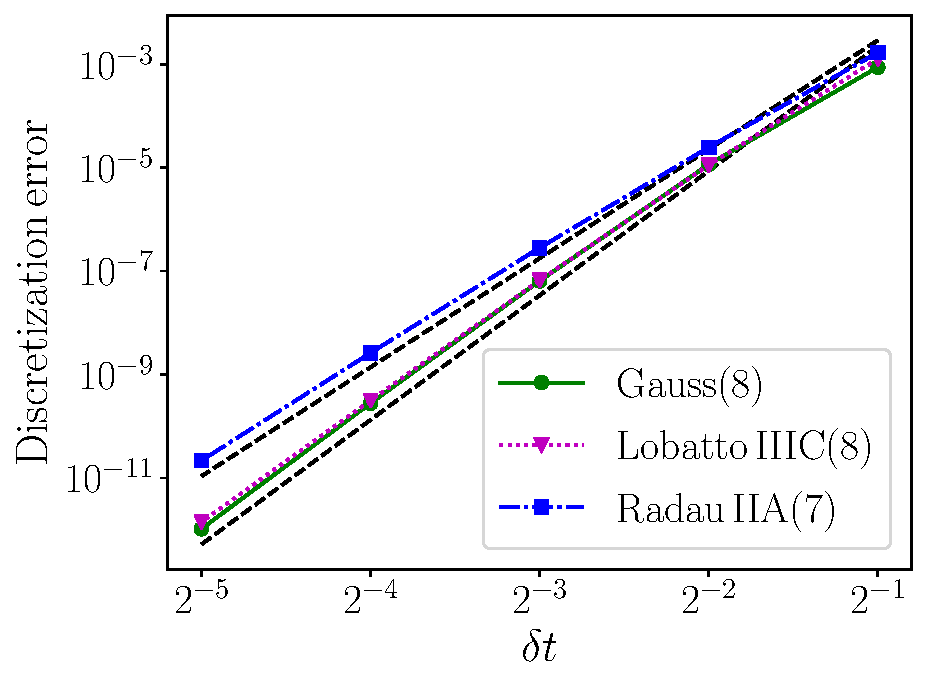
\includegraphics[width = 0.475\textwidth]{figures/FD_ex/errors_iters_18_38_27_d2_ex1.pdf}
\quad
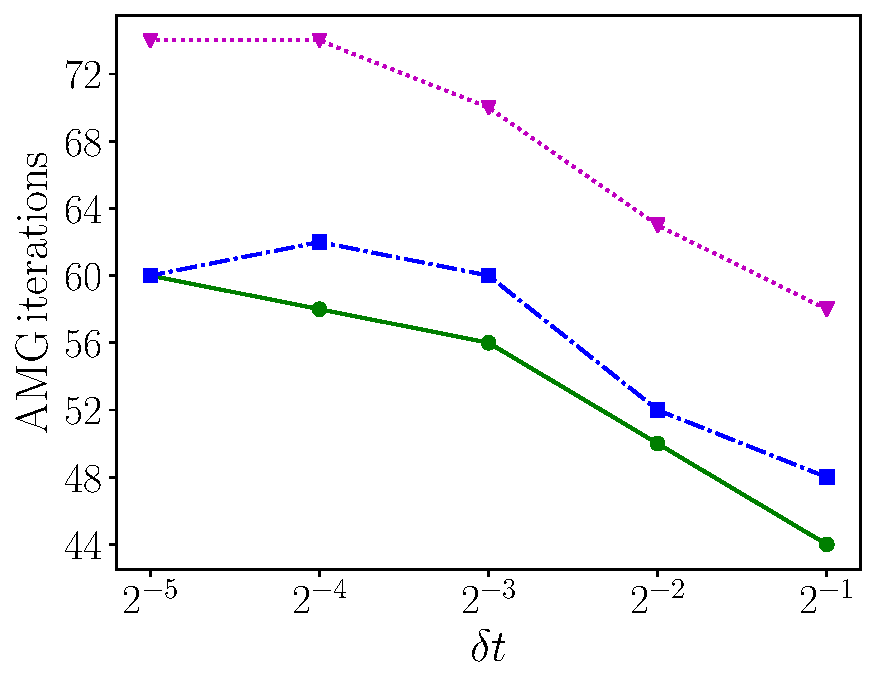
\includegraphics[width = 0.475\textwidth]{figures/FD_ex/amg_iters_18_38_27_d2_ex1.pdf}
}
\caption{Finite-difference advection-diffusion problem \eqref{eq:FD_ex}. $L_{\infty}$-discretization errors at $t = 2$ as a function of time-step $\delta t$ are shown on
the left for various discretizations of approximately 4th order (top) and 8th order (bottom). Black, dashed lines with slopes of three and four are shown (top), as are those with slopes of seven and eight (bottom). Plots on the right show the average number of AMG iterations per time step.
\label{fig:FD_ex}
}
\end{figure}

The preconditioner appears robust with respect to mesh and problem size, since
the average number of AMG iterations per time step (which is a proxy for the
number of GMRES iterations) remains roughly constant as the the mesh is refined.
Of the fully implicit methods, Gauss requires the fewest AMG iterations, closely
followed by Radau IIA methods, with the Lobatto IIC methods requiring the most
AMG iterations. This is
consistent with the theoretical estimates in Tables \ref{tab:beta} and \ref{tab:cond}.
Note that while Gauss and Radau IIA methods have very similar
iteration counts, Gauss converges at one order faster, which can be seen in the
left-hand panel of the figure.

Considering the lower-order methods in the top
row of Fig. \ref{fig:FD_ex}, L--SDIRK(4), a 5-stage, 4th-order, L-stable SDIRK
method requires the most AMG iterations of all methods. A--SDIRK(4), a 3-stage,
4th-order, A-stable SDIRK method, requires far fewer AMG iterations than
L--SDIRK(4). However, A--SDIRK(4) yields a significantly larger discretization
error than the other 4th-order schemes, and takes longer to reach its asymptotic
convergence rate. Thus, in terms of work done per accuracy, the new
preconditioner with 4th-order Gauss integration is the clear winner
for this particular test problem, requiring roughly half the AMG iterations
of the commonly used L-stable SDIRK4 scheme.

% ------------------------------------------------------------------------------------- %
% ------------------------------------------------------------------------------------- %
\subsection{DG advection(-diffusion)}\label{sec:numerics:dg}

This section considers a more difficult advection-diffusion problem, discretized
using a high-order DG finite element method. In particular, we demonstrate
the effectiveness and scalability of the new preconditioning on more complex flows and
DG discretizations (\Cref{fig:ad_advdiff} and \Cref{sec:numerics:dg:adv}),
the reduction in computational work that can be achieved using large time steps and
very high-order integration (\Cref{sec:numerics:dg:adv}), and how
using multiple ``inner'' preconditioning iterations to approximate $\widehat{L}^{-1}$
(or even inner Krylov acceleration) can be important for the fast, scalable
application of IRK integration (\Cref{sec:numerics:dg:diff}).

The governing equations in spatial domain $\Omega = [0,1] \times [0,1]$ are given by
\begin{equation} \label{eq:adv-diff}
	u_t + \nabla \cdot ( \bm\beta u  - \varepsilon \nabla u ) = f
\end{equation}
where $\bm\beta(x,y) : = (\cos(4\pi y), \sin(2 \pi x))^T$
is the velocity field and $\varepsilon$ the diffusion coefficient.
Periodic boundary conditions are enforced on $\partial\Omega$, and
\eqref{eq:adv-diff} is discretized with an upwind DG method \cite{Cockburn2001},
where diffusion terms are treated with the symmetric interior penalty method
\cite{Arnold1982,Arnold2002}. The resulting finite element problem is to find
$u_h \in V_h$ such that, for all $v_h \in V_h$,
\[
	\begin{multlined}
	\int_\Omega \partial_t (u_h) v_h \, dx
	- \int_\Omega u_h \bm\beta \cdot \nabla_h v_h \, dx
	+ \int_\Gamma \widehat{u_h} \bm\beta \cdot \llbracket v_h \rrbracket \, ds
	+ \int_\Omega \nabla_h u_h \cdot \nabla_h v_h \, d\bm x \\
	- \int_\Gamma \{ \nabla_h u_h \} \cdot \llbracket v_h \rrbracket \, ds
	- \int_\Gamma \{ \nabla_h v_h \} \cdot \llbracket u_h \rrbracket \, ds
	+ \int_\Gamma \sigma \llbracket u_h \rrbracket \cdot \llbracket v_h \rrbracket \, ds
	= \int_\Omega f v_h \, dx,
	\end{multlined}
\]
where $V_h$ is the DG finite element space consisting of piecewise polynomials of degree
$p$ defined on elements of the computational mesh $\mathcal{T}$ of the domain $\Omega$.
No continuity is enforced between mesh elements.
Here, $\nabla_h$ is the broken gradient, $\Gamma$ denotes the skeleton of the mesh,
and $\{ \cdot \}$ and $\llbracket \cdot \rrbracket$ denote the average and jump of a
function across a mesh interface.
$\widehat{u_h}$ is used to denote the upwind numerical flux.
This discretization has been implemented in the MFEM finite element framework
\cite{Anderson2020}, and uses AMG preconditioning with approximate ideal restriction
(AIR) \cite{Manteuffel:2019,Manteuffel:2018} (after first scaling by the DG
block-diagonal inverse).

The DG method is particularly advantageous for advection-dominated problems.
In the following subsections we vary $\varepsilon$ from $0$ (purely advective) to $0.01$.
The velocity field, initial condition, and numerical solution for $\varepsilon = 10^{-6}$
are shown in \Cref{fig:ad_advdiff}.

% srun -n32 ./dg_adv_diff  -rs 3 -rp 1 -i 18 -o 4 -dt 0.1 -air 2 -tf 10 -e 1e-6 -nov
% dt = 0.1, hmin = 0.015625, hmax = 0.015625
% time order = 8, space order = 4
% time acc. = 1e-08, space acc. = 5.96046e-08
%
\begin{figure}[!htb]
  \centering
  \begin{subfigure}[b]{0.3\textwidth}
    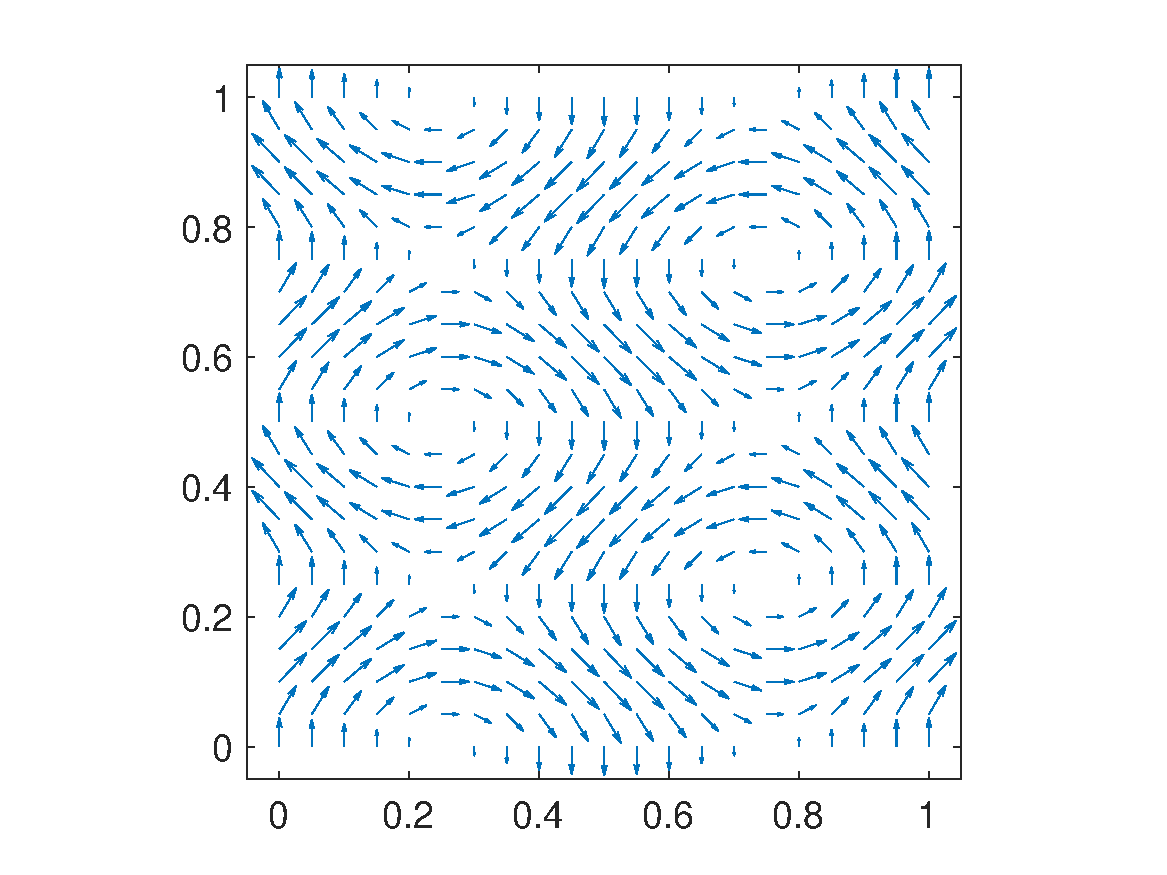
\includegraphics[width=\textwidth]{./figures/velocity_field.pdf}
    \caption{Velocity field}\label{fig:v}
  \end{subfigure}
   \begin{subfigure}[b]{0.3\textwidth}
    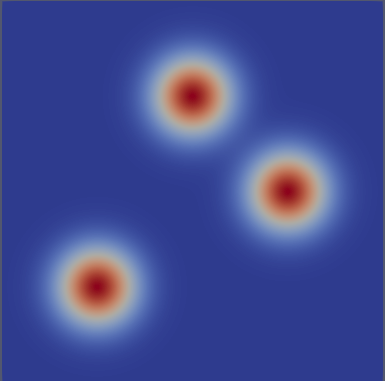
\includegraphics[width=\textwidth]{./figures/solution.0000.png}
    \caption{$t = 0$}
  \end{subfigure}
  \begin{subfigure}[b]{0.3\textwidth}
    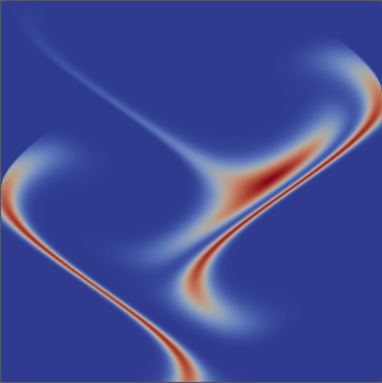
\includegraphics[width=\textwidth]{./figures/solution.0003.png}
    \caption{$t = 0.3$}
  \end{subfigure}
  \\\vspace{2ex}
   \begin{subfigure}[b]{0.3\textwidth}
    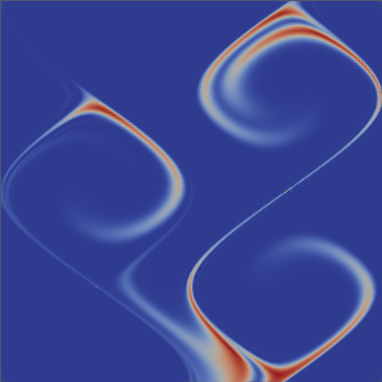
\includegraphics[width=\textwidth]{./figures/solution.0008.png}
    \caption{$t = 0.8$}
  \end{subfigure}
   \begin{subfigure}[b]{0.3\textwidth}
    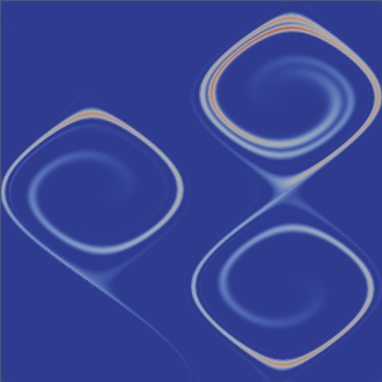
\includegraphics[width=\textwidth]{./figures/solution.0020.png}
    \caption{$t = 2.0$}
  \end{subfigure}
  \begin{subfigure}[b]{0.3\textwidth}
    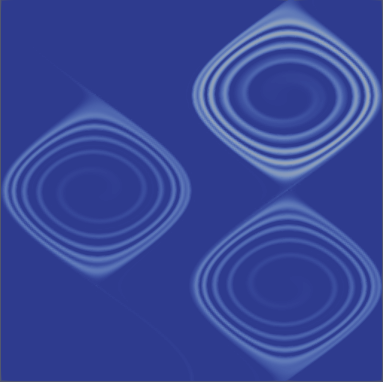
\includegraphics[width=\textwidth]{./figures/solution.0070.png}
    \caption{$t = 7.0$}
  \end{subfigure}
  \\\vspace{2ex}
      \caption{Advection-diffusion problem with velocity field shown in
      subplot (a) and the solution plotted for various time points from
      $t=0$ to $t = 7.0$ in subplots (b-f). Heatmap indicates solution in the
      2d domain, with blue $\mapsto 0$ and red $\mapsto 1$.}
  \label{fig:ad_advdiff}
\end{figure}

% ------------------------------------------------------------------------------------- %
\subsubsection{A hyperbolic example, and preconditioning with $\eta$ vs. $\gamma_*$}
\label{sec:numerics:dg:const}

First, we demonstrate the effectiveness of using $\gamma_*$ (\Cref{sec:solve:gamma})
instead of $\eta$ in the preconditioner, as well as the robustness of the proposed
method on a fully hyperbolic problem, where most papers have only discussed parabolic
PDEs. Thus, we set the diffusion coefficient $\varepsilon = 0$
and apply AIR as a preconditioner for individual systems
$(\gamma M - \delta t\mathcal{L})$.

AIR was originally designed for upwind DG discretizations of advection
and is well-suited for this problem. We use the \textit{hypre} implementation,
with distance 1.5 restriction with strength tolerance $\theta_R=0.01$, one-point
interpolation (type 100), Falgout coarsening (type 6) with strength tolerance
$\theta_C=0.1$, no pre-relaxation, and forward Gauss Seidel
post-relaxation (type 3), first on F-points followed by a second sweep on
all points. The domain is discretized using 4th-order finite elements on a
structured mesh, and the time step for each integration scheme is chosen
such that the spatial and temporal orders of accuracy match; for example,
for 8th-order integration we choose $\delta t = \sqrt{h}$, for mesh spacing
$h$, so that $\delta t^8 = h^4$. All linear systems are solved to a relative
tolerance of $10^{-12}$. There are a total of 1,638,400 spatial degrees-of-freedom
(DOFs), and the simulations are run on 288 processors on the Quartz machine at
Lawrence Livermore National Lab, resulting in $\sim$5600 DOFs/processor.

Table \Cref{tab:gamma} shows the average number of AIR iterations to solve for
each stage of an IRK method using $\eta$ and $\gamma_*$ as the preconditioning
constants. Iteration counts are shown for Gauss, Radau IIA, and Lobatto IIIC integration,
with 2-5 stages, and the (factor of) reduction in iteration count achieved using $\gamma_*$
vs. $\eta$ is also shown. For 5-stage Lobatto IIIC integration, $\gamma_*$ yields
almost a $6\times$ reduction in total inner AIR iterations to solve for the
``hard'' stage ($\beta > \eta$), while in no cases is there an increase in
iteration count when using $\gamma_*$.

{
% \renewcommand{\tabcolsep}{4pt}
\renewcommand{\arraystretch}{1.15}
\begin{table}[!ht]
  \centering
  \begin{tabular}{|l || r | rr | rr | rrr |}  % chktex 44
  \hline
\multicolumn{9}{|c|}{Gauss}\\\hline
Stages/Order & 2/4 & \multicolumn{2}{c}{3/6} & \multicolumn{2}{|c}{4/8} & \multicolumn{3}{|c|}{5/10} \\\hline
Iterations$(\eta)$ & 17 & 6 & 30 & 11  & 47 & 8 & 16 & 70 \\
Iterations$(\gamma_*)$ & 11 & 6 & 15 & 10 & 19 & 8 & 13 & 23 \\\hline
Speedup & 1.5 & 1.0 & 2.0 & 1.1 & 2.5 & 1.0 & 1.2 & 3.0 \\\hline\hline
\multicolumn{9}{|c|}{Radau IIA}\\\hline
Stages/Order & 2/3 & \multicolumn{2}{c}{3/5} & \multicolumn{2}{|c}{4/7} & \multicolumn{3}{|c|}{5/9} \\\hline
Iterations$(\eta)$ & 12 & 5 & 39 & 11 & 64 & 8 & 16 & 97 \\
Iterations$(\gamma_*)$ & 12 & 5 & 18 & 9 & 21 & 8 & 12 & 25 \\\hline
Speedup & 1.0 & 1.0 & 2.2 & 1.2 & 3.0 & 1.0 & 1.3 & 3.9 \\\hline\hline
\multicolumn{9}{|c|}{Lobatto IIIC}\\\hline
Stages/Order & 2/2 & \multicolumn{2}{c}{3/4} & \multicolumn{2}{|c}{4/6} & \multicolumn{3}{|c|}{5/8} \\\hline
Iterations$(\eta)$ & 8 & 3 & 67 & 11 & 113 & 7 & 17 & 175 \\
Iterations$(\gamma_*)$ & 8 & 3 & 22 & 9 & 26 & 7 & 12 & 30 \\\hline
Speedup & 1.0 & 1.0 & 3.0 & 1.2 & 4.3 & 1.0 & 1.4 & 5.8 \\\hline\hline
  \end{tabular}
  \caption{Average AIR iterations to solve for each stage in an implicit
  Runge-Kutta method using preconditioners $(\eta M - \mathcal{L})^{-2}$ and
  $(\gamma_* M - \mathcal{L})^{-2}$ \eqref{eq:gam_opt}. The ratio of
  iterations$(\eta)$/iterations$(\gamma_*)$ is shown in the ``Speedup'' rows.}
  \label{tab:gamma}
\end{table}
}


% ------------------------------------------------------------------------------------- %
\subsubsection{High-order \& advection-dominated}\label{sec:numerics:dg:adv}

This section demonstrates high-order IRK integration applied to the advection-dominated
problem in \Cref{fig:ad_advdiff}, using AIR as a preconditioner for the linear
systems.

\Cref{fig:dg_o4_abs} shows the total number of AIR iterations required to
compute one time step using six different Runge-Kutta schemes, from 4th
to 10th order, as a function of mesh spacing $h$. Note that as $h\to 0$,
there is only modest growth in the number of AIR iterations per time step,
indicating good (but not perfect) scalability.
Moreover, note that there is small growth in the number of iterations for
SDIRK4 as well (increasing from 20 to 25), which suggests the growth in
iteration count is due to imperfect scalability of AIR iterations rather
than the new IRK preconditioning.

\Cref{fig:dg_o4_rel} then shows the relative number of AIR iterations to
compute a given accuracy compared to SDIRK4. For example, if $h=0.01$,
then SDIRK4 uses $\delta t_4 = 0.01$ and Gauss8 uses $\delta t_8 =
\sqrt{0.01} = 0.1 = 10\delta t_4$, that is, $10\times$ less time steps to
achieve comparable accuracy. Note that as $h\to 0$, this factor becomes progressively
larger. For quite moderate $h$, we see how very high-order integration
can quickly lead to a reduction in total AIR iterations compared to a
standard SDIRK4 iteration. Gauss8 and Radau9, for example, require almost
$7\times$ less AIR iterations than SDIRK4 at $h =\delta t_4 = 1/256$,
and this ratio continues to decrease for smaller $\delta t$. Although this
does not account for additional setup time, where Gauss8 and Radau9 require
solving two different linear systems and SDIRK4 only one, very high-order
integration permitted through the new preconditioning still offers the
opportunity for significant speedups.

%
\begin{figure}[!h]
  \centering
  \begin{subfigure}[b]{0.475\textwidth}
    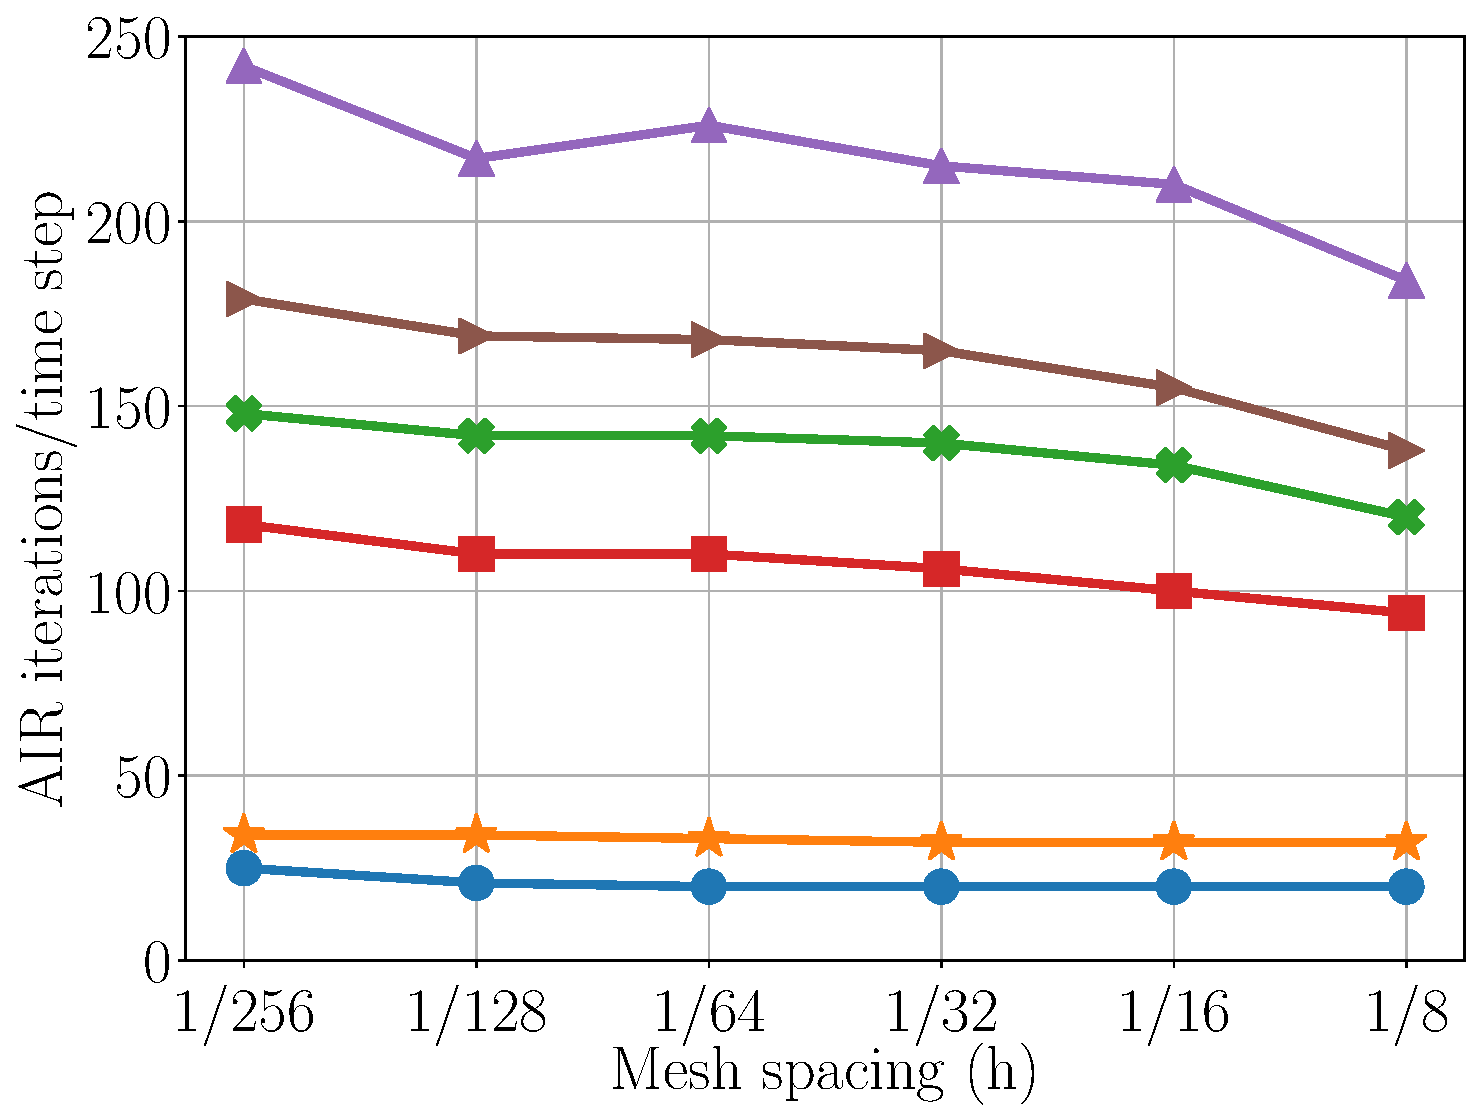
\includegraphics[width=\textwidth]{./figures/dg_advdiff_o4_1e-6.pdf}
    \caption{Total AIR iterations per time step}
	\label{fig:dg_o4_abs}
  \end{subfigure}
   \begin{subfigure}[b]{0.475\textwidth}
    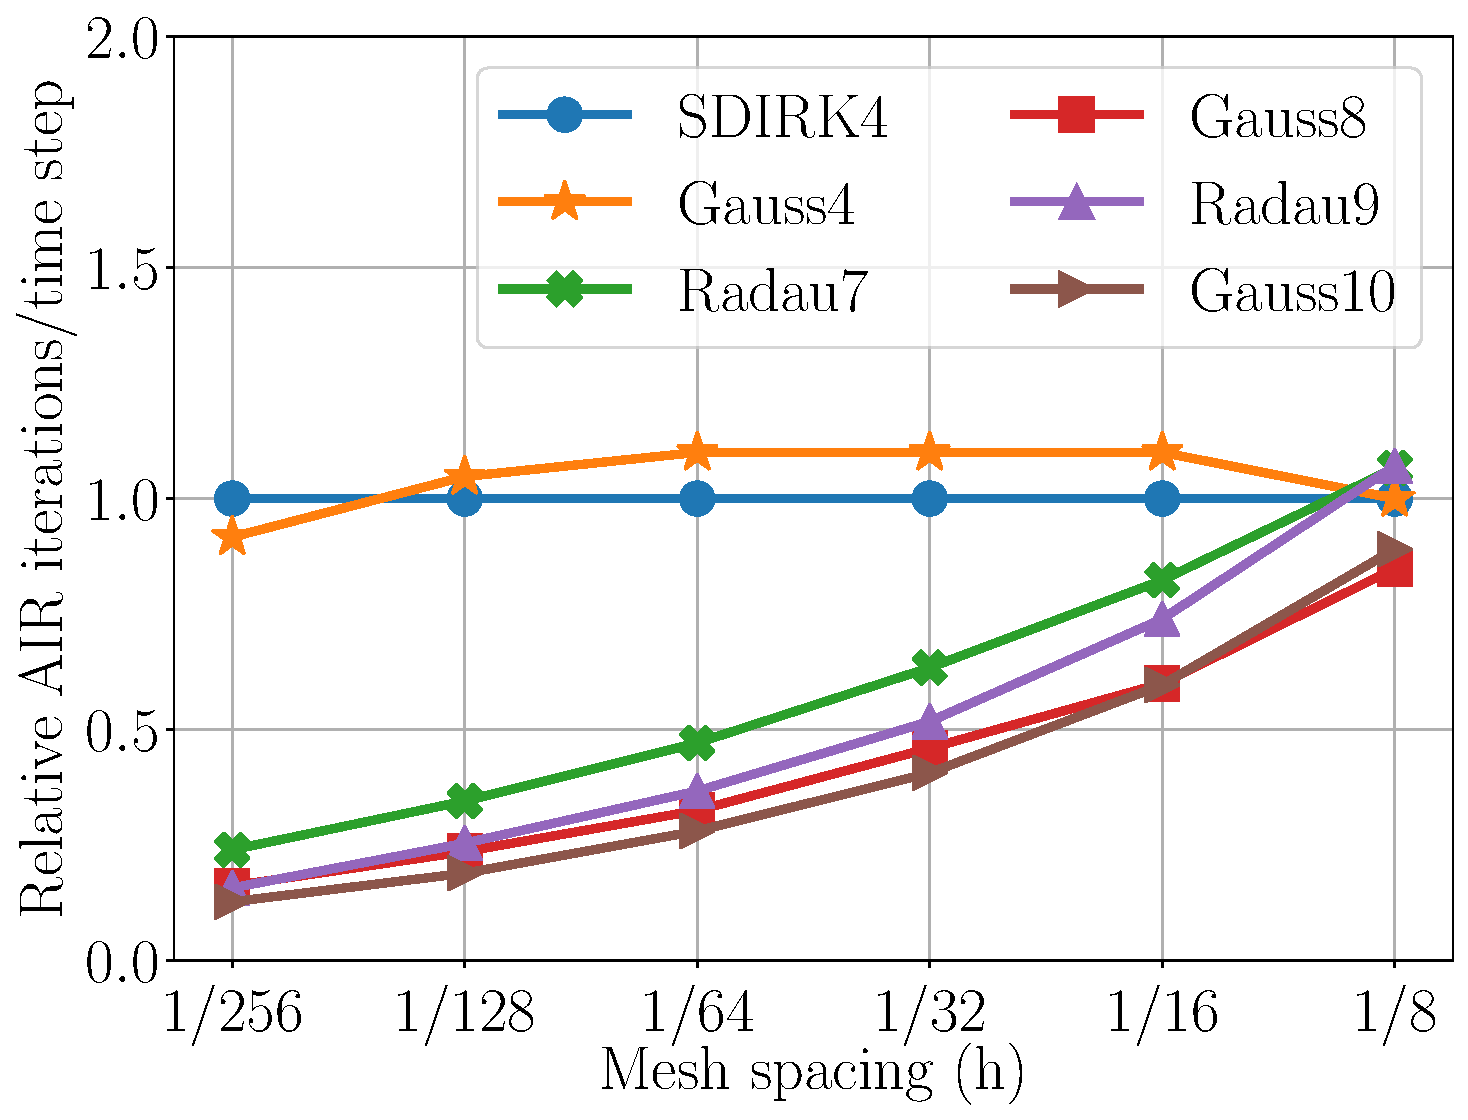
\includegraphics[width=\textwidth]{./figures/dg_advdiff_o4_1e-6_rel.pdf}
   \caption{AIR iterations relative to SDIRK4}
	\label{fig:dg_o4_rel}
  \end{subfigure}
\caption{}
  \label{fig:dg_o4}
\end{figure}
%


% ------------------------------------------------------------------------------------- %
\subsubsection{Diffusive problems and inner Krylov}\label{sec:numerics:dg:diff}

In \cite{AIR2}, AIR was shown to be effective on some DG advection-diffusion
problems, and classical AMG is known to be effective on diffusion-dominated
problems. However, the region of comparable levels of advection and diffusion
remains the most difficult from a multigrid perspective. We use this to
demonstrate how methods developed here require a ``good'' preconditioner
for a backward Euler time step in order to converge on more general IRK
methods. Fortunately, ensuring a preconditioner is sufficiently good can be
resolved by appealing to standard block preconditioning techniques, where an inner
iteration is used that applies multiple AIR iterations as a single preconditioner.

Here we consider an analogous problem to above, but set the diffusion coefficient
to $\varepsilon = 0.01$. We use a mesh with spacing $h \approx 0.001$, 2nd-order
DG finite elements, a time step of $\delta t = 0.1$, and three-stage 6th-order
Gauss integration. Altogether, this yields equal orders of accuracy, with time and
space error $\sim10^{-6}$. FGMRES \cite{saad1993flexible} is used for the
outer iteration, which allows for GMRES to be applied in an inner iteration
as a preconditioner for $(\gamma_* M - \mathcal{L})$. \Cref{fig:dg_o2} plots the
total number of AIR iterations per time step as a function of the number of
AIR iterations applied for each application of the preconditioner, using an
inner GMRES or an inner fixed-point iteration. An advection-dominated problem
with $\varepsilon = 10^{-6}$ is also shown for comparison.

Recall we have three stages, one of which is a single linear system corresponding
to a real eigenvalue, and the other corresponding to a pair of complex conjugate
eigenvalues, which we precondition as in \Cref{sec:solve}. The latter ends up being
the more difficult problem to solve -- for $\varepsilon =0.01$ (\Cref{fig:dg_o2_1e-2}),
the outer FGMRES iteration for the complex conjugate quadratic does not converge in
1000 iterations when using one AIR iteration as a preconditioner.
If two AIR iterations with GMRES are used as a preconditioner,
the FGMRES iteration converges in approximately 130 iterations, each of which
requires two applications of GMRES preconditioned with two AIR iterations,
yielding just over 500 total AIR iterations to converge. Further increasing
the number of AIR iterations per preconditioning yields nice convergence
using inner fixed-point or GMRES, with 150 and 112 total AIR iterations per
time step, respectively. In contrast, \Cref{fig:dg_o2_1e-6} shows that
additional AIR iterations for the advection-dominated case are generally
detrimental to overall computational cost (although the outer iteration
converges slightly faster, it does not make up for the additional linear
solves/iteration).

\begin{figure}[h!]
\centering

  \centering
  \begin{subfigure}[b]{0.475\textwidth}
	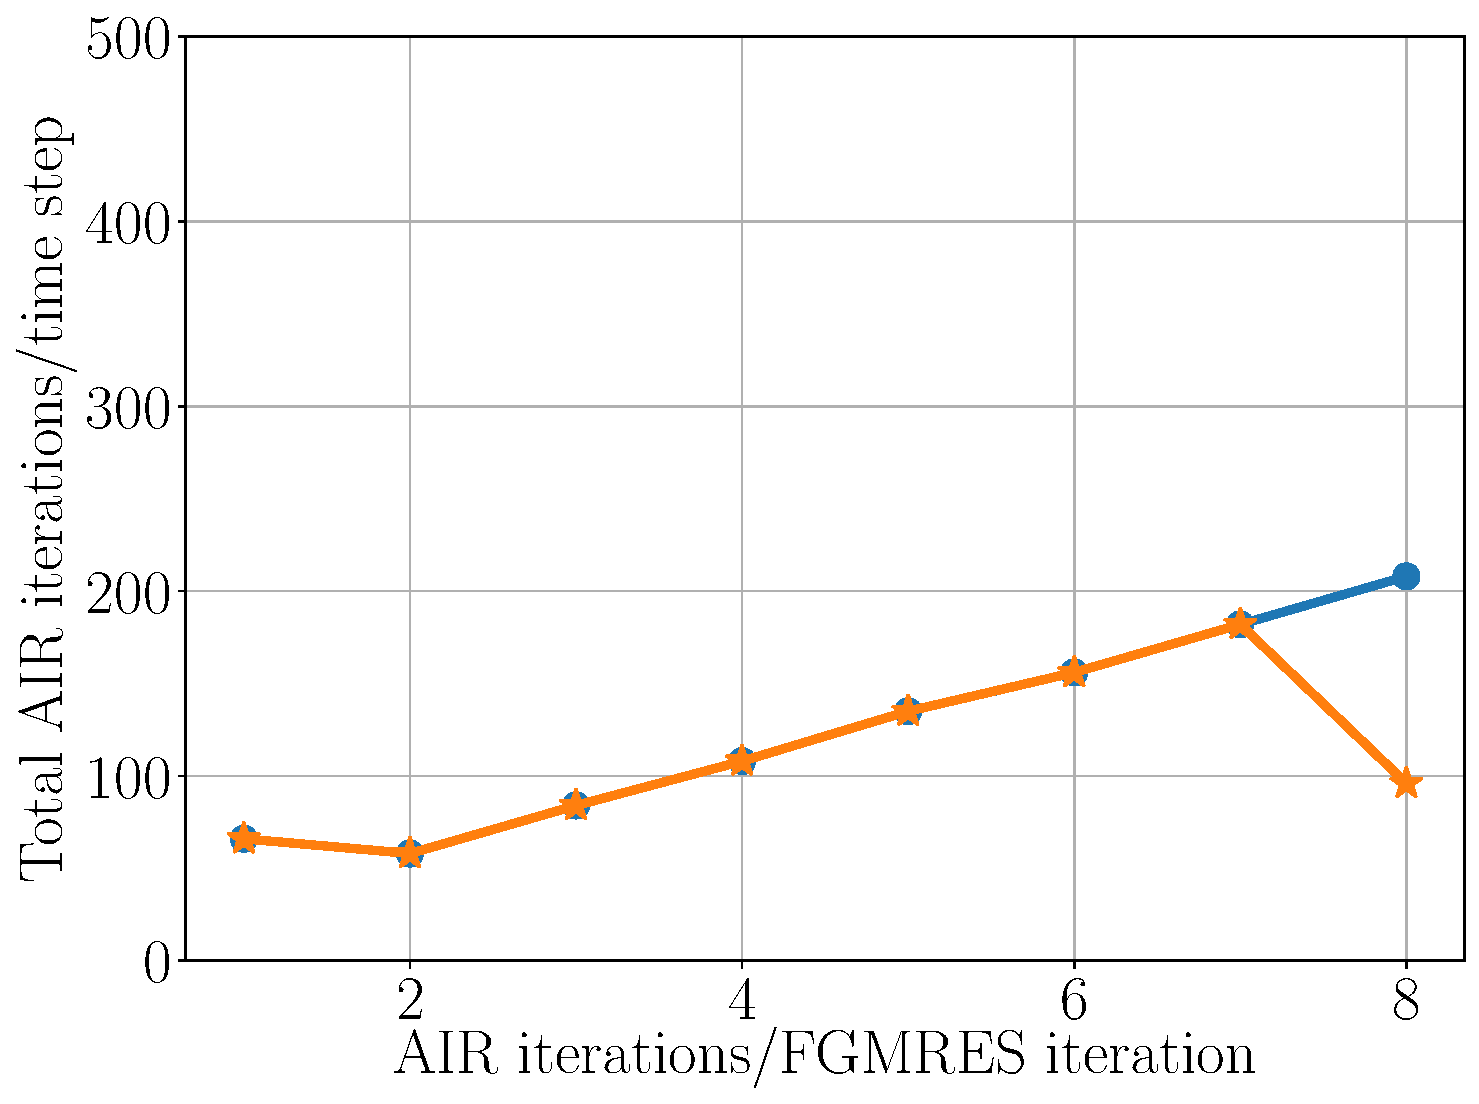
\includegraphics[width = \textwidth]{./figures/dg_advdiff_o2_1e-6.pdf}
	\caption{$\varepsilon = 10^{-6}$.}
	\label{fig:dg_o2_1e-6}
  \end{subfigure}
   \begin{subfigure}[b]{0.475\textwidth}
	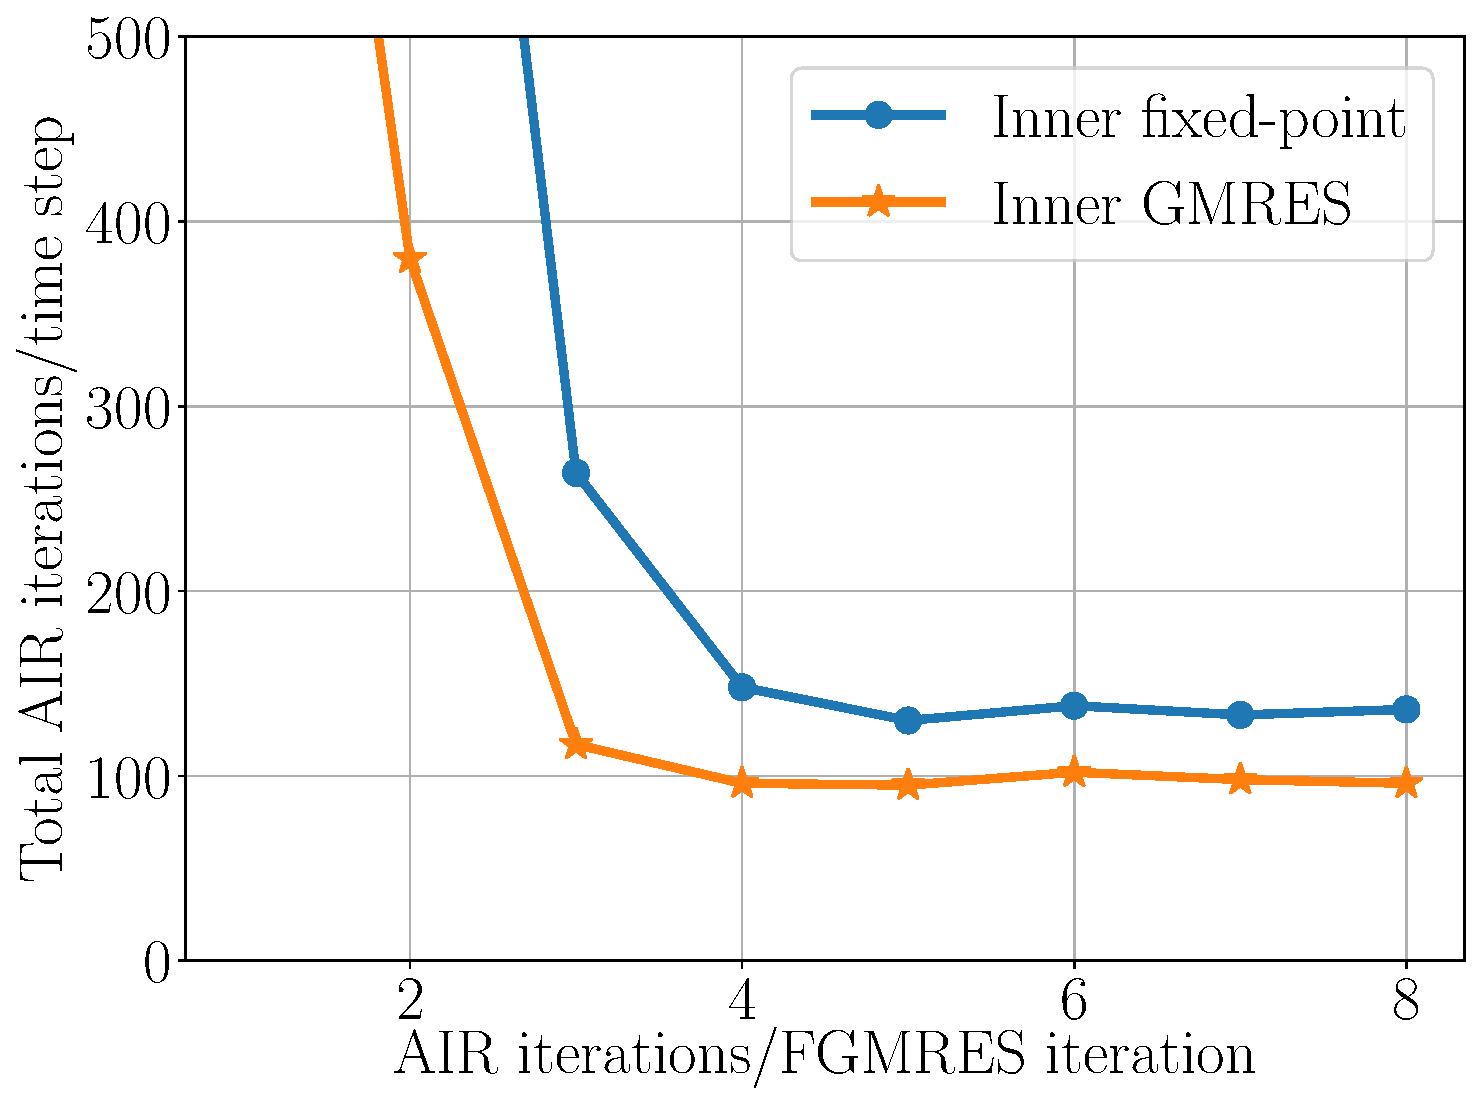
\includegraphics[width = \textwidth]{./figures/dg_advdiff_o2_1e-2.pdf}
	\caption{$\varepsilon = 0.01$.}
	\label{fig:dg_o2_1e-2}
  \end{subfigure}
\caption{AIR iterations per time step as a function of the number of
AIR iterations applied for each application of the preconditioner.}
\label{fig:dg_o2}
\end{figure}




% ------------------------------------------------------------------------------------- %
% ------------------------------------------------------------------------------------- %
\subsection{High-order matrix-free diffusion}

In this example, we illustrate the use high-order IRK methods coupled with high-order finite element spatial discretizations.
It is well-known that matrix assembly becomes prohibitively expensive for high-order finite elements.
Naive algorithms typically require $\mathcal{O}(p^{3d})$ operations to assemble the resulting system matrix, where $p$ is the polynomial degree and $d$ is the spatial dimension.
Techniques such as sum factorization can reduce this cost on tensor-product elements to $\mathcal{O}(p^{2d+1})$, however this cost can still be prohibitive for large values of $p$ \cite{Melenk2001}.
On the other hand, matrix-free operator evaluation on tensor-product meshes can be performed in $\mathcal{O}(p^{d+1})$ operations \cite{Orszag1980}, motivating the development of solvers and preconditioners that can be constructed and applied without access to the assembled system matrix \cite{Kronbichler2019}.

We consider a high-order finite element discretization of the linear heat equation on spatial domain $\Omega$,
\[
	\int_\Omega \partial_t (u_h) v_h \, dx + \int_\Omega \nabla u_h \cdot \nabla v_h \, dx = \int_\Omega f v_h \, dx,
\]
where $u_h, v_h \in V_h$, and $V_h$ denotes the degree-$p$ $H^1$-conforming finite element space defined on a mesh $\mathcal{T}$ consisting of tensor-product elements (i.e.\ quadrilaterals or hexahedra).
The matrix-free action of the corresponding operator is computed in $\mathcal{O}(p^{d+1})$ operations using the \textit{partial assembly} features of the MFEM finite element library \cite{Anderson2020}.
In order to precondition the resulting system, we make use of a low-order refined preconditioner, whereby the high-order system is preconditioned using a spectrally equivalent low-order finite element discretization computed on a refined mesh \cite{Canuto2010}.
The low-order refined discretization can be assembled in $\mathcal{O}(p^d)$ time, thereby avoiding the prohibitive costs of high-order matrix assembly.
We make use of the uniform preconditioners for the low-order refined problem based on subspace corrections, developed in \cite{Pazner2019a}.

For this test case, take the spatial domain to be $\Omega = [0,1] \times [0,1]$, with periodic boundary conditions.
We choose the forcing term
\[
	f(x, y, t) = \sin (2\pi x)\cos(2\pi y) \left(\cos(t) + 8 \pi^2 (2 + \sin(t)) \right),
\]
which corresponds to the exact solution
\[
	u(x, y, t) = \sin(2\pi x)\cos(2\pi y)(2 + \sin(t)).
\]
We begin with a very coarse $3 \times 3$ mesh, and integrate in time until $t=0.1$ using the Gauss and Radau IIA methods of orders 2 through 10.
For each test case, the finite element polynomial degree is set to $k-1$, where $k$ is the order of accuracy of the time integration method, resulting in $k$th order convergence in both space and time.
The mesh and time step are refined by factors of two to confirm the high-order convergence in space and time of the method.
The relative $L^2$ error, obtained by comparing against the exact solution, is shown in \Cref{fig:high-order-diff-errors}.

We also use this test case to study the effect of inner iterations on the convergence of the iteration solver.
As discussed in Section \ref{sec:inexact-precond}, it is important that the underlying preconditioner provide a good approximation of the inverse of the operator.
For that reason, we consider the use of an inner Krylov solver at every iteration.
Since this corresponds to using a variable preconditioner at each iteration, a flexible Krylov method may have be used for the outer iteration, although in practice good convergence is often still observed using the standard conjugate gradient method \cite{Notay2000}.
In particular, we compare the total number of preconditioner applications required to converge the outer iteration to a relative tolerance of $10^{-10}$, both with and without an inner Krylov solver.
For the inner Krylov solver, we use a conjugate gradient iteration with the same relative tolerance as the outer iteration in order to give a good approximation to the inverse of the operator.
The iteration counts are displayed in \Cref{fig:high-order-diff-iters}.
We note that for the fully implicit IRK methods, using an inner Krylov solver can reduce the total number of preconditioner applications by about a factor of 1.5, although this depends on the type of method and order of accuracy.
For DIRK methods, the use of inner iterations does not reduce the total number of preconditioner applications.
For this test case, the total number of preconditioner applications required for the second and fourth order Gauss IRK methods is between 1.3 and 2 times smaller than those required for the corresponding equal-order DIRK methods.

\begin{figure}
	\centering
	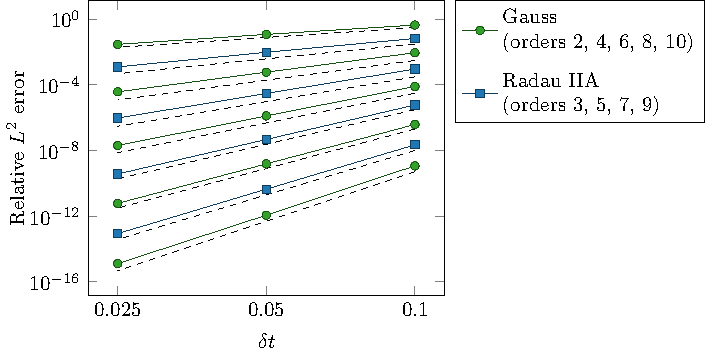
\includegraphics{figures/high_order_diff_error_plot/ho_diff_errors}
	\caption{
		High-order convergence in space and time for the matrix-free diffusion problem.
		Gauss and Radau IIA methods of orders 2 through 10 are used.
		The expected rates of convergence are recovered.
	}
	\label{fig:high-order-diff-errors}
\end{figure}

\begin{figure}
	\centering
	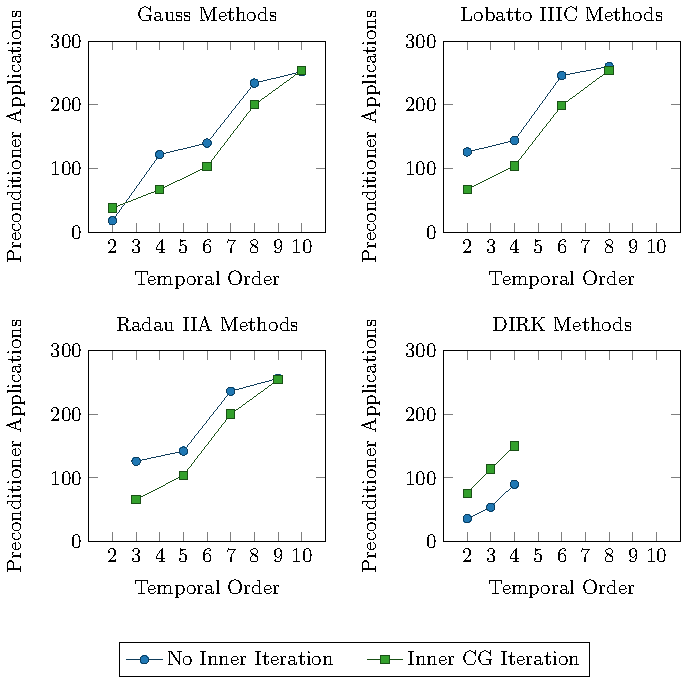
\includegraphics{figures/high_order_diff_iters/high_order_diff_iters}
	\caption{
		Comparison of number of iterations with and without inner iterations, using the high-order finite element diffusion test problem.
		Both the outer iteration and the inner conjugate gradient iteration are converged to a relative tolerance of $10^{-10}$.
	}
	\label{fig:high-order-diff-iters}
\end{figure}

% ------------------------------------------------------------------------------------- %
% ------------------------------------------------------------------------------------- %
% ------------------------------------------------------------------------------------- %
\section{Conclusions}\label{sec:conc}

This paper introduced a theoretical and algorithmic framework for the fast, parallel
solution of fully implicit Runge-Kutta methods in numerical PDEs (without algebraic
constraints). A field of values analysis is derived to guarantee rapid Krylov
convergence...\todo{finish}

% ------------------------------------------------------------------------------- %
\bibliographystyle{siamplain}
\bibliography{refs2.bib}


\end{document}
